\documentclass[12pt,a4paper]{report}

%% ── Packages ──────────────────────────────────────────────────────────────────
\usepackage[utf8]{inputenc}
\usepackage[T1]{fontenc}
\usepackage{mathptmx}   % Times New Roman (text + math)
\usepackage[margin=1in, headheight=15pt]{geometry}
\usepackage{graphicx}
\usepackage{float}
\usepackage{amsmath,amssymb}
\usepackage{algorithm}
\usepackage{algpseudocode}
\usepackage{booktabs}
\usepackage{multirow}
\usepackage{xcolor}
\usepackage{listings}
\usepackage{caption}
\usepackage{subcaption}
\usepackage{hyperref}
\usepackage{url}
\usepackage[round,authoryear]{natbib}
\usepackage{setspace}
\usepackage{fancyhdr}
\usepackage{titlesec}
\usepackage{enumitem}
\usepackage{pgfplots}
\pgfplotsset{compat=1.18}
\usepackage{tikz}
\usepackage{pifont}
\usetikzlibrary{shapes.geometric, arrows.meta, positioning, fit, backgrounds}

%% ── YAML language definition for listings ─────────────────────────────────────
\lstdefinelanguage{yaml}{
  keywords={true,false,null,yes,no},
  keywordstyle=\color{blue!70!black}\bfseries,
  comment=[l]{\#},
  commentstyle=\color{green!50!black},
  stringstyle=\color{red!70!black},
  morestring=[b]',
  morestring=[b]"
}

%% ── Formatting ────────────────────────────────────────────────────────────────
\singlespacing
\hypersetup{colorlinks=true, linkcolor=blue!70!black, citecolor=green!50!black, urlcolor=blue}

%% Page counter for "Page X of Y"
\usepackage{lastpage}

\pagestyle{fancy}
\fancyhf{}
\lhead{\small Page \thepage\ of \pageref{LastPage}}
\rhead{\small Siddiqi, Maaz}
\renewcommand{\headrulewidth}{0.4pt}

%% ── Code listing style ────────────────────────────────────────────────────────
\lstset{
  basicstyle=\ttfamily\footnotesize,
  breaklines=true,
  frame=single,
  backgroundcolor=\color{gray!8},
  keywordstyle=\color{blue!70!black}\bfseries,
  commentstyle=\color{green!50!black},
  stringstyle=\color{red!70!black},
  numbers=left,
  numberstyle=\tiny\color{gray},
  numbersep=8pt,
  captionpos=b
}

%% ─────────────────────────────────────────────────────────────────────────────
\begin{document}

%% ── Title Page ────────────────────────────────────────────────────────────────
\pagenumbering{roman}
\begin{titlepage}
  \thispagestyle{empty}
  \centering
  \vspace*{1.5cm}
  {\LARGE\bfseries
  Federated Learning over Heterogeneous Networks:\\[0.4em]
  A Network-Aware Simulator for Characterising QoS Impact\\[0.4em]
  on Model Convergence\par}
  \vspace{1.5cm}
  {\large Final Report -- Undergraduate Thesis\par}
  \vspace{1cm}
  {\large Maaz Siddiqi\par}
  \vspace{0.5cm}
  {\large CS 4490Z -- Thesis\par}
  \vspace{0.5cm}
  {\large Department of Computer Science\par}
  \vspace{0.5cm}
  {\large Western University\par}
  \vspace{0.5cm}
  {\large \today\par}
  \vspace{1cm}
  {\large Supervisor: Dr.\ Zubair Fadlullah, Dept.\ of Computer Science\par}
  \vspace{0.5cm}
  {\large Course Coordinator: Prof.\ Nazim Madhavji, Dept.\ of Computer Science\par}
\end{titlepage}

%% ── Glossary ──────────────────────────────────────────────────────────────────
\chapter*{Glossary}
\addcontentsline{toc}{chapter}{Glossary}

\begin{description}[leftmargin=3cm, style=nextline]
  \item[API] Application Programming Interface
  \item[CPU] Central Processing Unit
  \item[FL]  Federated Learning
  \item[HPC] High-Performance Computing
  \item[HTTP] Hypertext Transfer Protocol
  \item[IFB] Intermediate Functional Block
  \item[IID] Independent and Identically Distributed
  \item[JSON] JavaScript Object Notation
  \item[NIC] Network Interface Card
  \item[OOM] Out of Memory
  \item[QoS] Quality of Service
  \item[RAM] Random Access Memory
  \item[REST] Representational State Transfer
  \item[SGD] Stochastic Gradient Descent
  \item[TCP] Transmission Control Protocol
  \item[TLS] Transport Layer Security
  \item[VM]  Virtual Machine
  \item[WAN] Wide Area Network
  \item[YAML] YAML Ain't Markup Language
\end{description}

%% ── Abstract ──────────────────────────────────────────────────────────────────
\begin{abstract}
\addcontentsline{toc}{chapter}{Abstract}

\noindent\textbf{Background.}
Federated Learning (FL) enables collaborative model training without
centralising sensitive data, but its performance depends critically on
the network connecting participants---a dimension poorly served by
existing tools.  Network simulators such as NS-3 cannot execute real FL
algorithms, while FL frameworks such as Flower assume ideal network
conditions, leaving practitioners without a principled way to assess
whether a given network can support FL training.

\medskip
\noindent\textbf{Objectives.}
This thesis aims to (i)~design and implement a reproducible, open-source
Docker-based FL testbed with programmable network impairment injection;
(ii)~characterise how bandwidth, latency, and packet loss jointly affect
FL round duration and model convergence; and (iii)~derive a minimum
network requirement applicable to real-world FL deployments.

\medskip
\noindent\textbf{Methods.}
An open-source, Docker-based FL simulator was built, combining a real
FedAvg training loop (ResNet-18 on CIFAR-10, non-IID Dirichlet
$\alpha = 0.5$) with kernel-level network emulation via Linux
\texttt{tc netem}.  A systematic Quality of Service (QoS) parameter sweep
was conducted across five bandwidth levels (1--100~Mbps), three latency
values (5--200~ms), and three packet loss rates (0--5\%) over 20 FL
rounds with 3 clients, supplemented by scaling experiments (5 and 7
clients) and a straggler scenario.

\medskip
\noindent\textbf{Results.}
The experiments identify a throughput floor of $\beta^* \approx 3$~Mbps,
below which communication time exceeds training time and multi-round
convergence becomes impractical.  Bandwidth does not affect per-round
model accuracy: all configurations completing 18+ rounds converged to
65--67\% average accuracy, confirming that constrained bandwidth affects
training speed, not learning quality.  Packet loss at 5\% increased per-round upload time by $11\times$
(from 3.9\,s to 43\,s) and raised mean round duration by 16\%, but did
not prevent convergence; final accuracy of 67.8\% was consistent with
all other configurations.  Latency up to 200\,ms had negligible impact
($<$3\% increase in round duration).

\medskip
\noindent\textbf{Conclusions.}
These findings yield a practical client admission criterion
($\beta_k \geq 3$~Mbps) applicable to real-world FL deployments.
Clients with $\rho_k \approx 5\%$ can participate given adequate timeout
configuration, but impose an $11\times$ upload overhead and should be
treated as network stragglers.  The straggler effect---where one slow
client dominates round time---can be quantified and mitigated through
network-aware client selection.

\end{abstract}

\tableofcontents
\listoffigures
\listoftables

\pagenumbering{arabic}
%% ══════════════════════════════════════════════════════════════════════════════
\chapter{Introduction}
%% ══════════════════════════════════════════════════════════════════════════════

\section{Background and Motivation}

The proliferation of edge devices, smartphones, and institutional networks has generated
vast quantities of sensitive data, including medical records, biometric readings, and
usage patterns, that cannot practically or legally be centralised for training.
Federated Learning (FL), introduced by \citet{mcmahan2017communication},
addresses this by allowing a global model to be trained across many participants without
any raw data leaving its source. Each client trains locally and shares only model weight
updates with a central server, which aggregates them via the FedAvg algorithm and
redistributes an improved global model.

While FL's privacy guarantees are well-studied, a less-examined dimension is its
sensitivity to the network over which it operates. Every FL round requires each
participating client to download the current global model, train locally, and upload its
updated weights. For a model such as ResNet-18, with approximately 44 MB of parameters,
this represents significant data transfer repeated across every round of training.
In heterogeneous real-world deployments, clients may range from hospital servers on
gigabit ethernet to IoT devices on congested mobile links. The question of whether a
given network environment can sustain FL training, and how long it will take, is
practically important but poorly answered by existing tools.

Current network simulation and analysis platforms do not bridge this gap. Tools such as
OmNet++ and NS-3 are capable discrete-event network simulators, but they operate at the
packet level and require artificial traffic models to approximate ML workloads; real
neural network training cannot be executed inside them. MATLAB's network toolbox offers
mathematical modelling, but lacks the containerisation and Python ecosystem integration
needed to run production FL code. Vendor solutions such as Cisco's network analysis
platforms are closed ecosystems with no mechanism for plugging in arbitrary training
algorithms. FL frameworks themselves, such as Flower and TensorFlow Federated, run real
training but assume ideal network conditions and offer no facility for programmable
impairment injection.

This thesis presents an open-source, Docker-based FL simulator that closes this gap.
By combining a real FL training loop (ResNet-18 on CIFAR-10) with Linux traffic control (\texttt{tc netem})
applied inside each client container, the framework enables direct measurement of how
bandwidth, latency, and packet loss affect FL convergence, using real model weights,
real gradients, and real timing data. The result is a reproducible testbed that a
researcher or practitioner can use to characterise whether a given network environment
can support FL, and to estimate the time cost of training at scale.

\section{Problem Statement}

Existing FL implementations are typically validated under ideal, local network
conditions, such as Docker bridge networks on a single machine, that provide
effectively unlimited bandwidth and near-zero latency. This leaves open a
fundamental practical question for anyone considering a real-world FL deployment:

\begin{quote}
\emph{What is the minimum network capacity a federated client requires to
participate usefully in a training process, and how do bandwidth, latency,
and packet loss jointly affect convergence rate and final model accuracy?}
\end{quote}

Answering this question has two dimensions. The first is theoretical: given a
known model size, one can derive an expected upload time at any bandwidth and
estimate a floor below which round durations become impractical. The second is
empirical: TCP retransmission behaviour under packet loss, synchronisation
overhead, and straggler effects mean that real-world degradation diverges from
the clean theoretical prediction. No existing open tool allows both dimensions
to be measured together, with a real training algorithm and real model weights,
under programmatically controlled network conditions.

This thesis addresses that gap directly. The practical implications are
significant: FL deployment decisions, client selection policies, and resource
allocation on shared compute infrastructure all depend on having a principled,
measurable answer to the question above.

\section{Contributions}

The main contributions of this work are:
\begin{itemize}
  \item A fully reproducible, open-source Docker Compose FL testbed with integrated
        \texttt{tc netem} network emulation (Section~\ref{sec:impl}).
  \item Empirical characterisation of FL per-round communication cost under
        heterogeneous network conditions (Section~\ref{ch:qos}).
  \item A quantitative throughput-convergence model identifying the minimum
        effective bandwidth for stable FL training (Section~\ref{sec:results}).
  \item A practical minimum network requirement applicable to real-world FL
        deployments, derived from the empirical sweep results (Section~\ref{sec:future}).
\end{itemize}

\section{Thesis Structure}

The remainder of this thesis is organised as follows.
Chapter~\ref{ch:related} surveys related work in federated learning, existing
network simulation tools, and network-aware FL.
Chapter~\ref{ch:problem} formalises the system model, communication cost model,
and research questions.
Chapter~\ref{ch:method} describes the experimental methodology, including the FL
architecture, dataset and non-IID partitioning, network impairment model, evaluation
metrics, and experimental protocol.
Chapter~\ref{ch:impl} details the software implementation: repository structure,
Docker Compose orchestration, server and client design, and network emulation.
Chapter~\ref{ch:qos} presents the QoS analysis, including theoretical throughput
predictions and empirical convergence results.
Chapter~\ref{ch:future} discusses future research directions.
Chapter~\ref{ch:conclusion} concludes the thesis.

%% ══════════════════════════════════════════════════════════════════════════════
\chapter{Related Work}
\label{ch:related}
%% ══════════════════════════════════════════════════════════════════════════════

\section{Federated Learning}

Federated Learning was formally introduced by \citet{mcmahan2017communication},
who proposed the FedAvg algorithm: each client trains a local model for one or more
epochs and sends its updated weights to a central server, which aggregates them as a
weighted average proportional to local dataset size. FedAvg remains the dominant
aggregation scheme and is the algorithm used in this thesis.

Subsequent work identified statistical heterogeneity as a core challenge. When client
datasets follow different class distributions (non-IID data), local model updates can
diverge, slowing convergence or causing the global model to oscillate.
\citet{li2020fedprox} proposed FedProx, which adds a proximal regularisation term to
the local objective to limit client drift under heterogeneous data distributions.
Independently, \citet{li2020federated} surveyed the broader landscape of FL
challenges, identifying communication cost, privacy, and systems heterogeneity as the
three dominant open problems.

Communication efficiency has received dedicated attention. \citet{konevcny2016federated} proposed structured and sketched updates to reduce the
size of model transmissions, observing that upload cost dominates in typical FL
deployments. This observation is directly relevant to this thesis: with a ResNet-18
model producing approximately 44 MB of weight updates per round, upload bandwidth
is the primary network bottleneck under study.

\section{Existing Network Simulation Tools}

A number of general-purpose network simulation platforms exist, but none adequately
support FL research that requires both real model training and programmable network
impairment.

NS-3 \citep{ns3} and OmNet++ \citep{omnetpp} are widely used discrete-event network
simulators. Both model packet-level network behaviour with high fidelity, but they
operate independently of application logic. To simulate FL traffic in either tool, a
researcher must approximate model weight transfers as synthetic packet flows, losing
the real gradient dynamics, convergence behaviour, and timing characteristics of actual
training. Neither tool has native integration with Python-based ML frameworks such as
PyTorch or TensorFlow.

MATLAB's network simulation capabilities, available through Simulink and the
Communications Toolbox, are oriented toward signal-level and protocol-level modelling.
Running a distributed containerised workload with real model training inside MATLAB is
not practical, and the licensing cost limits reproducibility in academic settings.

Vendor platforms such as Cisco Packet Tracer and Cisco Modelling Labs are closed
ecosystems designed for configuring and testing network device behaviour. They provide
no mechanism for executing arbitrary application code or injecting a custom training
algorithm.

On the FL side, frameworks such as Flower \citep{beutel2020flower} and TensorFlow
Federated \citep{tff} enable real FL training but make the opposite trade-off: they
run real model updates while assuming ideal or real network conditions, with no
facility for programmatically injecting bandwidth limits, latency, or packet loss
across clients.

The result is a gap at the intersection of the two concerns: no existing open tool
allows a researcher to run a real FL training loop, with real model weights, under
fully programmable and reproducible network impairment.

\section{Network-Aware Federated Learning}

The impact of network conditions on FL has received growing attention.
\citet{lim2020federated} survey FL for mobile edge networks, identifying bandwidth
variability and device heterogeneity as primary obstacles to practical deployment.
\citet{nishio2019client} proposed FedCS, a client management
protocol that selects participants for each round based on estimated resource
availability, including network speed, to meet a round deadline.
\citet{lai2021oort} introduced Oort, which combines statistical utility with system
utility (including network throughput) to guide participant selection and improve
overall training efficiency.

These works share a common limitation: their network models are either analytical
approximations or drawn from real deployments that cannot be controlled or reproduced.
None provide empirical FL measurements under a systematic, programmable sweep of
network QoS parameters using real model training.

\section{Summary and Research Gap}

Existing work falls into two categories. Network simulators such as NS-3 and OmNet++
provide accurate packet-level modelling but cannot execute real FL algorithms.
FL frameworks such as Flower and TensorFlow Federated run real training but under
ideal or uncontrolled network conditions. Analytical studies of network-aware FL
propose client selection strategies without empirical validation under controlled
impairment.

This thesis bridges that gap. By combining a real FL training loop with kernel-level
network shaping via \texttt{tc netem} inside Docker containers, the framework presented
here enables direct, reproducible measurement of how bandwidth, latency, and packet
loss affect FL convergence with real model weights and real training dynamics.

%% ══════════════════════════════════════════════════════════════════════════════
\chapter{Research Goal and Objectives}
\label{ch:goals}
%% ══════════════════════════════════════════════════════════════════════════════

The overarching \textbf{goal} of this thesis is to empirically quantify the
impact of network Quality of Service (QoS) conditions on Federated Learning
(FL) convergence, and to derive a principled minimum network requirement that
practitioners can apply when deciding whether a client should participate in a
synchronous FL training process.

The following objectives operationalise this goal:

\begin{itemize}
  \item[\textbf{O1.}] Design and implement a reproducible, open-source
        Docker-based FL testbed with programmable network impairment injection
        via \texttt{tc netem}.
  \item[\textbf{O2.}] Characterise per-round communication cost as a function
        of model size and number of federated clients.
  \item[\textbf{O3.}] Conduct a systematic QoS parameter sweep across
        bandwidth, latency, and packet loss, and measure the effect on round
        duration and convergence speed.
  \item[\textbf{O4.}] Determine whether, and to what degree, network
        degradation below a threshold bandwidth affects final model accuracy in
        addition to training time.
  \item[\textbf{O5.}] Derive a minimum network requirement: a practical
        threshold below which a client should be excluded from synchronous FL
        rounds.
\end{itemize}

Together, O1 and O2 establish the experimental platform and its cost model;
O3 and O4 generate the empirical evidence; and O5 translates the findings into
a deployable decision criterion, directly attaining the stated goal.

%% ══════════════════════════════════════════════════════════════════════════════
\chapter{Problem Formulation}
\label{ch:problem}
%% ══════════════════════════════════════════════════════════════════════════════

\section{System Model}

Consider a federated learning system with one server $\mathcal{S}$ and a set of
$K$ clients $\mathcal{C} = \{c_1, c_2, \ldots, c_K\}$. Each client $c_k$ holds
a private local dataset $\mathcal{D}_k$ of $n_k$ labelled samples. The datasets
are non-overlapping across clients: $\mathcal{D}_i \cap \mathcal{D}_j = \emptyset$
for $i \neq j$.

A global model $f(\mathbf{x}; \boldsymbol{\theta})$ with parameters
$\boldsymbol{\theta}$ is trained collaboratively. In each training round $r$, every
client $c_k$ receives the current global parameters $\boldsymbol{\theta}^{(r)}$,
performs one epoch of local gradient descent on $\mathcal{D}_k$ to produce updated
parameters $\boldsymbol{\theta}_k^{(r)}$, and returns them to $\mathcal{S}$.
The server aggregates all client updates using the FedAvg rule:

\begin{equation}
  \boldsymbol{\theta}^{(r+1)} = \sum_{k=1}^{K} \frac{n_k}{n}
  \boldsymbol{\theta}_k^{(r)}
  \label{eq:fedavg}
\end{equation}

where $n = \sum_{k=1}^{K} n_k$ is the total number of training samples across
all clients. The updated global model $\boldsymbol{\theta}^{(r+1)}$ is then
redistributed to all clients for the next round.

\section{Communication Cost Model}

In standard federated learning, each client transmits and receives the full model
parameter vector each round. The per-round communication events for client $c_k$ are:

\begin{enumerate}
  \item \textbf{Model download:} receive $\boldsymbol{\theta}^{(r)}$ from
        $\mathcal{S}$, payload $B_w$ bytes.
  \item \textbf{Local training:} compute $\boldsymbol{\theta}_k^{(r)}$ over
        $\mathcal{D}_k$, duration $T_{\mathrm{train}}^{(k)}$.
  \item \textbf{Weight upload:} transmit $\boldsymbol{\theta}_k^{(r)}$ to
        $\mathcal{S}$, payload $B_w$ bytes.
\end{enumerate}

Since the same parameter vector is both downloaded and uploaded, the total bytes
exchanged by client $c_k$ per round is $B_{\mathrm{total}} = 2 B_w$. For the
ResNet-18 model used in this thesis, $B_w \approx 44.8$ MB, as confirmed by the
constant \texttt{submit\_bytes} value observed across all baseline runs.

The communication time for client $c_k$ over a channel with bandwidth $\beta_k$
(bps), one-way latency $\tau_k$ (ms), and packet loss rate $\rho_k$ is modelled as:

\begin{equation}
  T_{\mathrm{comm}}^{(k)} =
  \frac{B_{\mathrm{total}}}{\beta_k \cdot (1 - \rho_k)} + \alpha \cdot \tau_k
  \label{eq:tcomm}
\end{equation}

where $\alpha$ is a multiplier capturing the number of TCP round-trips incurred by
the HTTP-based model exchange protocol. The total wall-clock duration of round $r$
is governed by the \emph{straggler}, the client that takes longest to complete.
Under synchronous FedAvg, the server cannot aggregate until every client has
submitted its update, so:

\begin{equation}
  T_{\mathrm{round}}^{(r)} = \max_{k \in \mathcal{C}}
  \left( T_{\mathrm{train}}^{(k)} + T_{\mathrm{comm}}^{(k)} \right)
  \label{eq:tround}
\end{equation}

Equation~\ref{eq:tround} makes the straggler effect explicit: a single
bandwidth-constrained client can dominate $T_{\mathrm{round}}$ regardless of how
fast all other clients are. This motivates the search for a minimum bandwidth
threshold below which including a client becomes counterproductive.

\section{Research Questions}

Three formal research questions are derived from the system model above:

\begin{description}
  \item[RQ1 (Throughput Floor):] Is there a minimum bandwidth $\beta^*$ such that
  for $\beta_k < \beta^*$, client $c_k$ becomes a straggler that causes
  $T_{\mathrm{round}}$ to grow super-linearly, making synchronous FL impractical?

  \item[RQ2 (Accuracy Degradation):] Does operating below $\beta^*$ also reduce
  final model accuracy after $R$ rounds, or is the effect purely on training time?

  \item[RQ3 (Minimum Network Requirement):] Can a simple threshold defined over
  $\beta_k$, $\tau_k$, and $\rho_k$ identify clients that should be excluded from
  a round in order to protect convergence integrity and bound round duration?
\end{description}

\section{Scope and Assumptions}

This thesis makes the following assumptions:
\begin{itemize}
  \item Synchronous FL aggregation via FedAvg; asynchronous FL is left for future work.
  \item TCP transport layer via HTTP; alternative protocols such as gRPC are
        not considered.
  \item Network conditions are stationary within a round but vary across experimental
        configurations.
  \item $K = 3$ clients in the main QoS sweep experiments; $K = 5$ and
        $K = 7$ in supplementary scaling experiments.
  \item ResNet-18 trained on CIFAR-10 (10-class image classification).
  \item Each client trains for $E = 1$ local epoch per round.
  \item Network shaping is applied to egress (upload) traffic only.  The
        configured bandwidth, latency, and packet loss affect model uploads from
        clients to the server; downloads are unthrottled due to the absence of
        the IFB kernel module on macOS Docker Desktop.  Symmetric and asymmetric
        ingress shaping are left for future work on native Linux hosts.
\end{itemize}

%% ══════════════════════════════════════════════════════════════════════════════
\chapter{Methodology}
\label{ch:method}
%% ══════════════════════════════════════════════════════════════════════════════

\section{Federated Learning Architecture}

The system follows the standard client-server FL topology.  A single server
$\mathcal{S}$ holds the global model and $K$ clients each hold a private local
dataset.  Communication is over HTTP/JSON on a shared Docker bridge network; the
server exposes a lightweight REST API and all model weight payloads are
serialised as raw byte buffers via \texttt{torch.save}.

Figure~\ref{fig:round_lifecycle} illustrates the five phases of each FL round.
The round boundary is defined by the server: it increments a global round counter
only after aggregation, and clients poll this counter to detect when the new
global model is available.  Because FedAvg is synchronous, the server blocks
aggregation until all $K$ clients have submitted their updates, creating the
straggler sensitivity formalised in Equation~\ref{eq:tround}.

\begin{figure}[H]
\centering
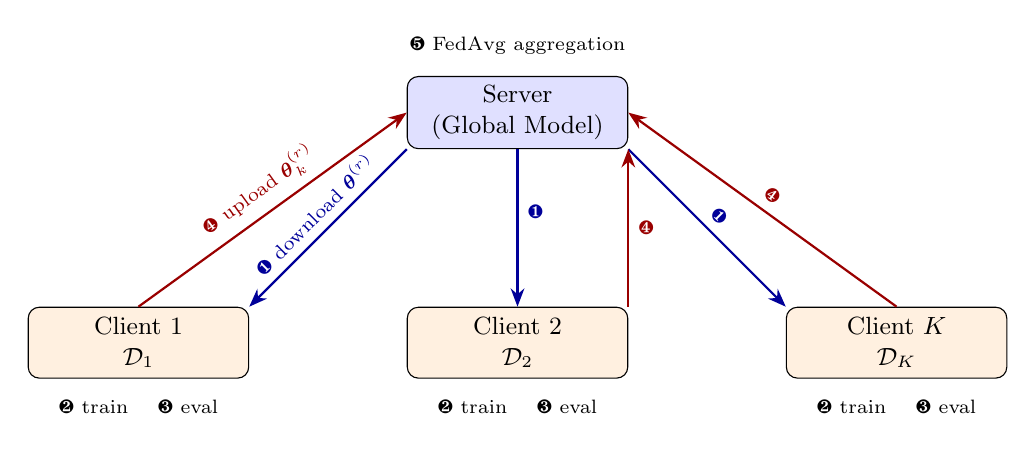
\begin{tikzpicture}[
  node distance=1.4cm and 3.5cm,
  box/.style={rectangle, draw, rounded corners, minimum width=2.8cm,
              minimum height=0.9cm, align=center, font=\small},
  lbl/.style={font=\scriptsize, midway},
  >=Stealth
]
  \node[box, fill=blue!12] (server) {Server\\(Global Model)};
  \node[box, fill=orange!12, below left=2.0cm and 2.0cm of server] (c1) {Client 1\\$\mathcal{D}_1$};
  \node[box, fill=orange!12, below=2.0cm of server] (c2) {Client 2\\$\mathcal{D}_2$};
  \node[box, fill=orange!12, below right=2.0cm and 2.0cm of server] (ck) {Client $K$\\$\mathcal{D}_K$};

  \draw[->, thick, blue!60!black] (server.south west) -- (c1.north east)
    node[lbl, above, sloped] {\ding{182} download $\boldsymbol{\theta}^{(r)}$};
  \draw[->, thick, blue!60!black] (server.south) -- (c2.north)
    node[lbl, right, pos=0.4] {\ding{182}};
  \draw[->, thick, blue!60!black] (server.south east) -- (ck.north west)
    node[lbl, above, sloped] {\ding{182}};

  \draw[->, thick, red!60!black] (c1.north) -- (server.west)
    node[lbl, above, sloped] {\ding{185} upload $\boldsymbol{\theta}_k^{(r)}$};
  \draw[->, thick, red!60!black] (c2.north east) -- (server.south east)
    node[lbl, right, pos=0.5] {\ding{185}};
  \draw[->, thick, red!60!black] (ck.north) -- (server.east)
    node[lbl, above, sloped] {\ding{185}};

  \node[font=\scriptsize, below=0.15cm of c1] {\ding{183} train \quad \ding{184} eval};
  \node[font=\scriptsize, below=0.15cm of c2] {\ding{183} train \quad \ding{184} eval};
  \node[font=\scriptsize, below=0.15cm of ck] {\ding{183} train \quad \ding{184} eval};

  \node[font=\scriptsize, above=0.15cm of server] {\ding{186} FedAvg aggregation};
\end{tikzpicture}
\caption{Per-round lifecycle: \ding{182}~model download,
  \ding{183}~local training, \ding{184}~local evaluation,
  \ding{185}~weight upload, \ding{186}~server aggregation.}
\label{fig:round_lifecycle}
\end{figure}

\section{Dataset and Data Heterogeneity}

All experiments use the CIFAR-10 benchmark \citep{krizhevsky2009learning}, which
contains 60{,}000 colour images of size $32 \times 32$ pixels across 10 classes
(airplane, automobile, bird, cat, deer, dog, frog, horse, ship, truck).  The
standard split provides 50{,}000 training images and 10{,}000 test images.
CIFAR-10 was chosen because it is well-understood, small enough to train on CPU
within Docker containers, and widely used in FL research, making results
comparable to prior work.

The model is a standard ResNet-18 \citep{he2016deep} with the final
fully-connected layer adjusted to output 10 classes.  The serialised model
weights occupy approximately 44.8~MB, which defines the per-round upload and
download payload $B_w$ used throughout the communication cost model
(Section~\ref{ch:problem}).

\subsection{Non-IID Partitioning via Dirichlet Distribution}

In real FL deployments, each client's data follows a different class distribution.
To emulate this statistical heterogeneity, the training set is partitioned across
$K$ clients using a Dirichlet distribution over class labels, following the
method of \citet{hsu2019measuring}.

For each of the 10 classes, the fraction of that class's samples assigned to each
client is drawn from $\mathrm{Dir}(\alpha)$, where $\alpha > 0$ is a
concentration parameter.  Low values of $\alpha$ produce highly skewed
distributions (some clients see only a few classes), while high values approach
uniform (IID) partitioning.

All experiments in this thesis use $\alpha = 0.5$, which produces moderate
heterogeneity: each client sees most classes but with substantially different
proportions.  This is consistent with the default used in recent FL
benchmarks and creates a realistic challenge for FedAvg convergence.

\begin{table}[H]
\centering
\caption{Effect of the Dirichlet concentration parameter $\alpha$ on data
         distribution across clients.}
\label{tab:alpha}
\begin{tabular}{cl}
\toprule
$\alpha$ & Effect on client data distribution \\
\midrule
0.1  & Highly non-IID: each client dominated by 1--2 classes \\
0.5  & Moderately non-IID: unequal proportions across all classes (\textbf{used}) \\
1.0  & Mildly non-IID: noticeable variation but all classes present \\
$\infty$ & IID: each client has a uniform class distribution \\
\bottomrule
\end{tabular}
\end{table}

\section{Network Impairment Model}

Network conditions are emulated using the Linux Traffic Control (\texttt{tc})
subsystem with the \texttt{netem} queueing discipline, which is the standard
kernel-level mechanism for injecting bandwidth limits, latency, and packet loss
on a per-interface basis.

Each client container runs with the \texttt{NET\_ADMIN} Docker capability.
Before the Python process starts, an entrypoint script applies a \texttt{tc netem}
rule to egress (upload) traffic:

\begin{itemize}
  \item \textbf{Egress (upload):} a \texttt{netem} qdisc is attached to
        \texttt{eth0} with the configured bandwidth rate, delay, and loss
        percentage.
\end{itemize}

Ingress (download) traffic is \emph{not} shaped.  Shaping ingress on Linux
requires an Intermediate Functional Block (IFB) kernel module, which is
unavailable on macOS Docker Desktop (LinuxKit VM).  Since all experiments in
this thesis were conducted on macOS, the configured impairment applies only to
the upload direction; downloads from the server are effectively unthrottled.
This is an acceptable simplification because the dominant communication cost in
FedAvg is the upload of model updates, which are the same size as the
downloaded global model but occur on the shaped path.  Containers with no
shaping configured skip the \texttt{tc} commands entirely, providing a clean
baseline.

Table~\ref{tab:sweep} lists the QoS parameter sweep used in all experiments.
Each experiment configuration fixes one dimension and varies another while
holding the third constant, producing a total of $5 + 3 + 3 = 11$ distinct
configurations (with the baseline shared across sweeps).

\begin{table}[H]
\centering
\caption{QoS parameter sweep space.  Bold values indicate the baseline.}
\label{tab:sweep}
\begin{tabular}{lll}
\toprule
Parameter & Values & Held constant at \\
\midrule
Bandwidth & 1, 5, 10, 50, \textbf{100} Mbps & $\tau = 5$ ms, $\rho = 0\%$ \\
Latency   & \textbf{5}, 50, 200 ms           & $\beta = 100$ Mbps, $\rho = 0\%$ \\
Packet loss & \textbf{0}, 1, 5\%              & $\beta = 100$ Mbps, $\tau = 5$ ms \\
\bottomrule
\end{tabular}
\end{table}

The bandwidth range spans from severely constrained (1~Mbps, representative of a
congested mobile link) to the unthrottled Docker bridge baseline (100~Mbps).
Latency values represent local (5~ms), regional (50~ms), and intercontinental
(200~ms) links.  Packet loss at 5\% represents a degraded wireless channel.

\section{Evaluation Metrics}

Each client and the server collect per-round statistics.
Table~\ref{tab:metrics} defines the full set of metrics recorded.

\begin{table}[H]
\centering
\caption{Per-round metrics collected during each experiment.}
\label{tab:metrics}
\begin{tabular}{llp{7.5cm}}
\toprule
Metric & Source & Definition \\
\midrule
\texttt{get\_model\_ms} & client &
  Wall-clock time (ms) to download the global model via \texttt{GET /model}. \\
\texttt{submit\_ms} & client &
  Wall-clock time (ms) for the \texttt{POST /update} request carrying the
  updated weight payload. Measured from request start to HTTP response; does
  not include polling or the subsequent model download. \\
\texttt{train\_ms} & client &
  Wall-clock time (ms) for one epoch of local SGD training. \\
\texttt{wait\_ms} & client &
  Idle time (ms) spent polling for round completion after submitting.
  Computed as $T_{\mathrm{wall}} - T_{\mathrm{get}} - T_{\mathrm{train}} -
  T_{\mathrm{submit}}$, capturing how long a fast client waits for stragglers. \\
\texttt{submit\_bytes} & client &
  Size (bytes) of the serialised model weights uploaded.  Constant at
  $\approx 44.8$~MB for ResNet-18. \\
\texttt{poll\_count} & client &
  Number of \texttt{GET /round\_status} polls before the round advances. \\
\texttt{wire\_tx\_bytes} & client &
  Total bytes transmitted at the NIC level (from \texttt{/sys/class/net/eth0/statistics/tx\_bytes}).
  Includes TCP headers, retransmissions, and ACKs. \\
\texttt{wire\_rx\_bytes} & client &
  Total bytes received at the NIC level.  Comparing
  \texttt{wire\_tx\_bytes} to \texttt{submit\_bytes} quantifies
  retransmission overhead under packet loss. \\
\texttt{duration\_ms} & server &
  Wall-clock time (ms) from receiving the first client update to completing
  FedAvg aggregation for the round. \\
accuracy / loss & client &
  Validation accuracy (\%) and cross-entropy loss evaluated on the client's
  local held-out split after loading the aggregated global model. \\
\bottomrule
\end{tabular}
\end{table}

Two derived metrics are used in the analysis:
\begin{itemize}
  \item \textbf{Retransmission overhead}: $\texttt{wire\_tx\_bytes} /
        \texttt{submit\_bytes}$, expected to be $\approx 1.0$ at 0\% loss and to
        grow with increasing packet loss.
  \item \textbf{Rounds to convergence} $R^*$: the first round at which the
        running-average validation accuracy (window of 3 rounds) plateaus within
        1 percentage point for 3 consecutive rounds.
\end{itemize}

\section{Experimental Protocol}

Each point in the QoS parameter sweep (Table~\ref{tab:sweep}) is executed as an
independent experiment run following Algorithm~\ref{alg:sweep}.  The automation
script \texttt{run\_experiment.py} generates a Docker Compose file from a YAML
configuration, builds the container image, starts all services, and collects
logs after the run completes.

\begin{algorithm}[H]
\caption{QoS Sweep Protocol}
\label{alg:sweep}
\begin{algorithmic}[1]
\Require Parameter grid $\mathcal{G} = \{(\beta, \tau, \rho)\}$, number of
         rounds $R = 20$, number of clients $K = 3$
\For{each $(\beta, \tau, \rho) \in \mathcal{G}$}
  \State Generate experiment YAML with $(\beta, \tau, \rho)$, $R$, $K$
  \State Generate Docker Compose file from YAML
  \State Build container image (cached if unchanged)
  \State Start server container; wait for healthcheck
  \State Start $K$ client containers with \texttt{tc netem} applied at boot
  \For{$r = 0$ \textbf{to} $R - 1$}
    \State Each client: download $\boldsymbol{\theta}^{(r)}$, train, upload
           $\boldsymbol{\theta}_k^{(r)}$
    \State Server: aggregate via FedAvg when all $K$ updates received
    \State Each client: poll until round advances, download new model, evaluate
    \State Record all metrics (Table~\ref{tab:metrics}) for round $r$
  \EndFor
  \State Collect per-client stats summaries from container logs
  \State Tear down all containers and network
\EndFor
\State Aggregate results across all configurations for analysis
\end{algorithmic}
\end{algorithm}

All experiments are run on a single host machine with containers sharing CPU
resources, eliminating hardware variability.  Network impairment is the only
controlled variable between configurations.  The CIFAR-10 dataset is downloaded
once and cached in a Docker volume shared across runs.

%% ══════════════════════════════════════════════════════════════════════════════
\chapter{Software Implementation}
\label{ch:impl}

\section{System Overview}
\label{sec:impl}

The implementation is organised as a Python monorepo with three top-level
concerns cleanly separated: application logic (\texttt{src/}), container
infrastructure (\texttt{infra/}), and experiment definitions
(\texttt{experiments/}).  The project is managed with \texttt{uv} and all
dependencies are pinned in \texttt{requirements.txt}.  Listing~\ref{lst:repo}
shows the directory layout.

\begin{lstlisting}[language=bash, caption={Repository structure (key files).},
  label=lst:repo]
project-root/
+-- src/
|   +-- server_main.py          # server entrypoint
|   +-- client_main.py          # client entrypoint
|   +-- fl/
|   |   +-- server_core.py      # FLServer: round mgmt + FedAvg
|   |   +-- client_core.py      # LocalTrainer: train + eval
|   |   +-- aggregation.py      # fed_avg()
|   +-- models/
|   |   +-- resnet.py           # ResNet-18 (10-class)
|   +-- data/
|   |   +-- cifar10.py          # CIFAR-10 + Dirichlet partition
|   +-- transport/
|   |   +-- interface.py        # abstract ServerTransport / ClientTransport
|   |   +-- http_adapter.py     # FastAPI server + httpx client
|   |   +-- serialization.py    # torch.save / torch.load wrappers
|   +-- stats/
|       +-- collector.py        # RoundStats + StatsCollector
|       +-- netio.py            # NIC tx/rx byte reader
+-- infra/
|   +-- Dockerfile.ml-base      # container image definition
|   +-- scripts/
|   |   +-- entrypoint.sh       # tc netem + exec
|   |   +-- generate_compose.py # YAML config -> compose.generated.yml
|   |   +-- run_experiment.py   # build + up + teardown orchestrator
+-- experiments/
    +-- baseline.yaml
    +-- heterogeneous.yaml
    +-- straggler.yaml
    +-- qos-sweep-bw.yaml
    +-- scale-5.yaml / scale-7.yaml
\end{lstlisting}

A central design decision is \textbf{transport-agnostic layering}.  The
FL logic---model aggregation (\texttt{FLServer}), local training
(\texttt{LocalTrainer}), and FedAvg (\texttt{fed\_avg})---is completely
decoupled from the communication mechanism.  Two abstract interfaces,
\texttt{ServerTransport} and \texttt{ClientTransport}
(\texttt{transport/interface.py}), define the contract between the FL
core and any transport implementation.  The current codebase provides an
HTTP+JSON adapter (\texttt{http\_adapter.py}), but the interface could
be satisfied by gRPC, WebSockets, or any other protocol without modifying
the training code.  This separation ensures that the QoS measurements
reported in Chapter~\ref{ch:qos} reflect the transport layer in
isolation, independent of training logic.

\section{Docker Compose Architecture}

Each experiment is executed inside a set of Docker containers orchestrated
by Docker Compose.  A code-generation step translates a declarative
experiment YAML file into a Compose file, ensuring that every run is
fully specified and reproducible.

\subsection{Container Image}

All containers---both server and clients---share a single image built from
\texttt{Dockerfile.ml-base}.  The image is based on
\texttt{python:3.10-slim} and installs the \texttt{iproute2} package
(which provides the \texttt{tc} utility for network shaping), along with
\texttt{curl} for the server healthcheck.  Application code is not baked
into the image; instead, the repository root is bind-mounted at
\texttt{/app} at runtime, so rebuilds are only needed when dependencies
change.  The image's entrypoint is \texttt{entrypoint.sh}, which applies
network shaping before starting the Python process
(Section~\ref{sec:netem}).

\subsection{Compose Generation}

The script \texttt{generate\_compose.py} reads an experiment YAML file
and produces \texttt{infra/compose.generated.yml}.
Listing~\ref{lst:yaml} shows an example experiment configuration; the
generated Compose file is excerpted in Listing~\ref{lst:compose}.

\begin{lstlisting}[language=yaml, caption={Experiment configuration
  (\texttt{heterogeneous.yaml}).}, label=lst:yaml]
experiment:
  name: "heterogeneous"
  rounds: 3
  num_clients: 3
  alpha: 0.5      # Dirichlet concentration

server:
  port: 8000

clients:
  - id: 1
    network: { bandwidth: "100mbit", latency: "5ms", loss: "0%" }
  - id: 2
    network: { bandwidth: "100mbit", latency: "5ms", loss: "1%" }
  - id: 3
    network: { bandwidth: "100mbit", latency: "5ms", loss: "0%" }
\end{lstlisting}

The generator creates one \texttt{fl-server} service and one
\texttt{fl-client-\textit{k}} service per client, all attached to a
shared bridge network (\texttt{fl-net}).  Network shaping parameters are
passed as environment variables (\texttt{TC\_BANDWIDTH},
\texttt{TC\_LATENCY}, \texttt{TC\_LOSS}) that the entrypoint script
reads at boot.  Every container is given the \texttt{NET\_ADMIN}
capability, which authorises the \texttt{tc} commands.  Client containers
declare a \texttt{depends\_on} healthcheck on the server, ensuring that
the FL server's HTTP API is reachable before any client starts training.

\begin{lstlisting}[language=yaml, caption={Excerpt from a generated
  \texttt{compose.generated.yml}.}, label=lst:compose]
services:
  fl-server:
    image: phase1-fl-ml:latest
    cap_add: [NET_ADMIN]
    environment:
      - ROLE=server
      - FL_SERVER_PORT=8000
      - NUM_CLIENTS=3
      - FL_ROUNDS=3
    healthcheck:
      test: ["CMD", "curl", "-f", "http://localhost:8000/health"]
    volumes: ["..:/app"]
    command: ["python", "-m", "src.server_main"]

  fl-client-1:
    image: phase1-fl-ml:latest
    cap_add: [NET_ADMIN]
    environment:
      - ROLE=client
      - CLIENT_ID=1
      - FL_SERVER_URL=http://fl-server:8000
      - TC_BANDWIDTH=100mbit
      - TC_LATENCY=5ms
      - TC_LOSS=0%
    depends_on:
      fl-server: { condition: service_healthy }
    volumes: ["..:/app"]
    command: ["python", "-m", "src.client_main"]
\end{lstlisting}

\section{FL Server}

The server is started by \texttt{server\_main.py}, which builds a
ResNet-18 model, wraps it in an \texttt{FLServer} instance, and hands
it to an \texttt{HTTPServerTransport}.  Table~\ref{tab:api} lists the
HTTP endpoints exposed by the server.

\begin{table}[H]
\centering
\caption{FL server REST API.}
\label{tab:api}
\begin{tabular}{llp{8cm}}
\toprule
Endpoint & Method & Description \\
\midrule
\texttt{/health} & GET &
  Returns \texttt{\{status: ok, round: $r$\}}.  Used by the Docker
  healthcheck and by clients to wait for readiness. \\
\texttt{/model} & GET &
  Returns the current global model weights as a binary
  \texttt{application/octet-stream} payload ($\approx 44.8$~MB for
  ResNet-18).  The body is produced by \texttt{torch.save}. \\
\texttt{/update/\{client\_id\}} & POST &
  Accepts a client's updated weights as a binary body.  When all $K$
  clients for the current round have submitted, FedAvg aggregation is
  triggered synchronously.  Returns \texttt{\{status: accepted,
  submitted\_round: $r$\}}. \\
\texttt{/round\_status} & GET &
  Returns \texttt{\{round: $r$, pending: $p$, expected: $K$\}}.
  Clients poll this endpoint to detect when aggregation has completed
  and the round counter has advanced. \\
\bottomrule
\end{tabular}
\end{table}

\subsection{Aggregation Logic}

The core aggregation is implemented in \texttt{FLServer.submit\_update()}:
each call appends the client's state dict to a pending list and checks
whether all $K$ updates have arrived.  When the list is full, the
private \texttt{\_aggregate()} method computes FedAvg (an unweighted
average across all client state dicts), loads the result into the global
model, clears the pending list, and increments the round counter.  The
round counter is the single source of truth for round progress---clients
detect round completion by polling \texttt{/round\_status} and comparing
the server's round number against the round they submitted for.

The server also records \texttt{duration\_ms} for each round, measured
from the first update received to the completion of aggregation.  This
captures both the straggler wait and the aggregation compute time.  After
all rounds complete, the server's \texttt{done\_event} is set, causing
the main thread to log a summary and shut down.

\section{FL Client}

Each client is started by \texttt{client\_main.py}, which parses
arguments from environment variables (injected by Docker Compose), waits
for the server healthcheck, loads its CIFAR-10 partition, and enters the
training loop.  The per-round control flow is:

\begin{enumerate}
  \item \textbf{Capture pre-round NIC counters.}  The function
        \texttt{read\_interface\_bytes("eth0")} reads the kernel
        \texttt{/sys/class/net/eth0/statistics/tx\_bytes} and
        \texttt{rx\_bytes} counters.  These are sampled before and after
        the round to compute \texttt{wire\_tx\_bytes} and
        \texttt{wire\_rx\_bytes}.

  \item \textbf{Download global model.}  \texttt{GET /model} fetches the
        latest global weights.  The client records
        \texttt{get\_model\_ms} and anchors the round wall-clock timer.

  \item \textbf{Local training.}  The \texttt{LocalTrainer} deep-copies
        the model, runs $E = 1$ epoch of SGD (Adam optimiser) over the
        client's local CIFAR-10 partition, and returns the updated state
        dict along with training loss and accuracy.  The elapsed time is
        recorded as \texttt{train\_ms}.

  \item \textbf{Upload update.}  \texttt{POST /update/\{client\_id\}}
        sends the serialised state dict.  The HTTP POST timeout is set
        to \texttt{None} (unlimited), since a bandwidth-constrained
        client may take several minutes to upload 44.8~MB.  The elapsed
        time from request start to HTTP response is recorded as
        \texttt{submit\_ms}.

  \item \textbf{Poll for aggregation.}  After the POST returns, the
        client polls \texttt{GET /round\_status} at 0.5\,s intervals
        until the server's round counter advances past the submitted
        round.  Each poll increments \texttt{poll\_count}.  Once the
        round is complete, the client fetches the new global model and
        records the full round wall-clock time, from which
        \texttt{wait\_ms} is derived.

  \item \textbf{Evaluate.}  The client evaluates the new global model on
        its local held-out validation split and logs accuracy and loss.

  \item \textbf{Capture post-round NIC counters.}  A second call to
        \texttt{read\_interface\_bytes} provides the delta, which is
        stored as \texttt{wire\_tx\_bytes} and \texttt{wire\_rx\_bytes}
        for the round.
\end{enumerate}

After all rounds complete (or an error terminates the loop early), the
client logs a summary table of all per-round metrics.

\subsection{Data Loading and Non-IID Partitioning}

The module \texttt{src/data/cifar10.py} provides a
\texttt{get\_client\_loaders()} function that downloads the CIFAR-10
dataset (cached in the container's filesystem), applies the Dirichlet
non-IID partitioning described in Section~\ref{ch:method}, and returns a
\texttt{(train\_loader, val\_loader)} pair for the specified client ID.
The partition is deterministic for a given seed, ensuring reproducibility
across runs.  A \texttt{--synthetic} flag is available for smoke tests:
it substitutes small random tensors, bypassing the dataset download
entirely.

\subsection{Statistics Collection}

Per-round metrics are managed by the \texttt{StatsCollector} class,
which maintains a list of \texttt{RoundStats} dataclass instances.
Each \texttt{RoundStats} holds \texttt{get\_model\_ms},
\texttt{submit\_ms}, \texttt{train\_ms}, \texttt{wait\_ms},
\texttt{submit\_bytes}, \texttt{poll\_count}, \texttt{wire\_tx\_bytes},
and \texttt{wire\_rx\_bytes}.  The \texttt{wait\_ms} field is derived
automatically: once the full round wall-clock time is known,
$\texttt{wait\_ms} = T_{\mathrm{wall}} - \texttt{get\_model\_ms} -
\texttt{train\_ms} - \texttt{submit\_ms}$, capturing the idle time a
fast client spends waiting for stragglers to finish.

\section{Network Emulation}
\label{sec:netem}

Network impairment is applied inside each client container at boot time,
before the Python process starts.  The container's entrypoint script
(\texttt{entrypoint.sh}) checks whether any \texttt{TC\_*} environment
variables are set and, if so, applies egress-only shaping.
Listing~\ref{lst:netem} shows the relevant command.

\begin{lstlisting}[language=bash, caption={Network shaping command from
  \texttt{entrypoint.sh}.}, label=lst:netem]
# Egress (upload) shaping on eth0
tc qdisc add dev eth0 root netem \
    delay ${TC_LATENCY} rate ${TC_BANDWIDTH} loss ${TC_LOSS}
\end{lstlisting}

A \texttt{netem} queueing discipline is attached to \texttt{eth0},
throttling all outgoing (upload) traffic.  Download traffic is not
shaped: Linux \texttt{tc} cannot directly throttle incoming packets
without an Intermediate Functional Block (IFB) kernel module, which is
unavailable inside the LinuxKit VM used by macOS Docker Desktop.
Because all experiments were run on macOS, only egress shaping is
applied.  In practice this means model uploads are throttled while
model downloads from the server proceed at full container network speed.
Since upload and download payloads are the same size in FedAvg, the
upload leg dominates observed round time under constrained bandwidth.

If none of the \texttt{TC\_*} variables are set, the script skips all
shaping and executes the Python process directly, providing a clean
unimpaired baseline.  The \texttt{NET\_ADMIN} Docker capability is
required for all \texttt{tc} commands; it is granted in the generated
Compose file.

\section{Observed Baseline Results}

The baseline experiment ($\beta = 100$~Mbps, $\tau = 5$~ms, $\rho = 0\%$,
$K = 3$, 20 rounds) establishes reference values for all metrics.  Key
observations from client-3's per-round data:

\begin{itemize}
  \item \textbf{Constant payload.}  \texttt{submit\_bytes} =
        44{,}803{,}531 bytes ($\approx$44.8~MB) every round, confirming
        that full model weights are transferred regardless of training
        outcome.
  \item \textbf{Fast uploads at baseline.}  \texttt{submit\_ms}
        $\approx$3.9\,s per round (model upload), with
        \texttt{get\_model\_ms} $\approx$0.2\,s (download is unthrottled).
  \item \textbf{Minimal wire overhead.}  $\texttt{wire\_tx\_bytes} /
        \texttt{submit\_bytes} \approx 1.01$, confirming negligible
        retransmission at 0\% loss.
  \item \textbf{Convergence.}  Validation accuracy progressed from
        42.6\% (round~0) to 72.4\% (round~19) for client-3; the 3-client
        average reached 66.4\% by round~18.
  \item \textbf{Training dominance.}  \texttt{train\_ms} $\approx$280\,s
        accounts for $\approx$97\% of the round wall-clock time at
        baseline, confirming that communication cost is negligible at
        100~Mbps.
\end{itemize}

%% ══════════════════════════════════════════════════════════════════════════════
\chapter{QoS Analysis and Results}
\label{ch:qos}
%% ══════════════════════════════════════════════════════════════════════════════

\section{Theoretical Throughput Analysis}
\label{sec:model}

Before running experiments, we can derive the expected communication time
from first principles.  The serialised ResNet-18 state dict is
$B_w = 44{,}797{,}387$ bytes ($\approx 44.8$~MB), which is constant
across all rounds and clients (confirmed empirically by the
\texttt{submit\_bytes} metric).  Because only egress (upload) traffic is
shaped, the upload direction is the bottleneck; downloads from the
server traverse the unthrottled ingress path and complete in negligible
time relative to the shaped upload.

The minimum theoretical upload time at bandwidth $\beta$ (bits per
second) with packet loss $\rho$ is:
\begin{equation}
  T_{\mathrm{xfer}}(\beta, \rho) = \frac{8 \times B_w}{\beta \times (1 - \rho)}
  \label{eq:xfer_time}
\end{equation}

The per-round communication time (excluding training) is dominated by
the upload:
\begin{equation}
  T_{\mathrm{comm}} \approx T_{\mathrm{upload}} + \alpha \cdot \tau
  = T_{\mathrm{xfer}}(\beta, \rho) + \alpha \cdot \tau
  \label{eq:tcomm_applied}
\end{equation}

where $\tau$ is one-way latency and $\alpha$ accounts for TCP handshake
round-trips and HTTP request/response overhead.  The download term is
omitted because ingress traffic is not shaped (see
Section~\ref{sec:netem}).

Table~\ref{tab:theory} applies Equation~\ref{eq:xfer_time} across the
bandwidth sweep at $\rho = 0\%$ to predict upload time per round.

\begin{table}[H]
\centering
\caption{Theoretical minimum upload time per round at each bandwidth
  ($B_w = 44.8$~MB, $\rho = 0\%$).  Download is unthrottled.}
\label{tab:theory}
\begin{tabular}{rrrl}
\toprule
$\beta$ (Mbps) & Upload (s) & Comm.\ time (s) & Practical? \\
\midrule
  1   & 358.4 & $\approx$358 & Impractical ($>$5 min/round) \\
  5   &  71.7 & $\approx$72  & Marginal ($>$1 min/round) \\
 10   &  35.8 & $\approx$36  & Marginal \\
 50   &   7.2 & $\approx$7   & Feasible \\
100   &   3.6 & $\approx$4   & Baseline \\
\bottomrule
\end{tabular}
\end{table}

Several observations follow from this analysis:

\begin{itemize}
  \item At 1~Mbps, a single round requires over 11 minutes of pure data
        transfer alone, before accounting for TCP overhead, training
        time, or polling.  Over 20 rounds, this amounts to nearly 4
        hours of communication cost.
  \item The communication-to-computation ratio shifts dramatically across
        the bandwidth range.  At 100~Mbps, training ($\approx 5$~s)
        dominates; at 1~Mbps, communication is $>$70$\times$ longer
        than training.
  \item The theoretical prediction does \emph{not} account for TCP
        retransmission overhead under packet loss, congestion window
        dynamics, or HTTP framing overhead.  Empirical measurements
        (Section~\ref{sec:bw_results}) are expected to exceed these
        lower bounds.
\end{itemize}

Based on this analysis, a \textbf{throughput floor} is predicted near
$\beta^* \approx 10$--$50$~Mbps.  Below 10~Mbps, per-round
communication time exceeds one minute even under ideal conditions,
making multi-round convergence prohibitively slow for synchronous
FedAvg with a 44.8~MB payload.

\section{Convergence Results}
\label{sec:results}

This section presents the empirical results from the QoS parameter sweep
defined in Section~\ref{ch:method}.  Each subsection isolates one
network parameter while holding the others at their baseline values.

\subsection{Effect of Bandwidth on Convergence}
\label{sec:bw_results}

Figure~\ref{fig:convergence_bw} plots validation accuracy against FL
round number for each bandwidth level in the sweep ($\tau = 5$~ms,
$\rho = 0\%$).

\begin{figure}[H]
\centering
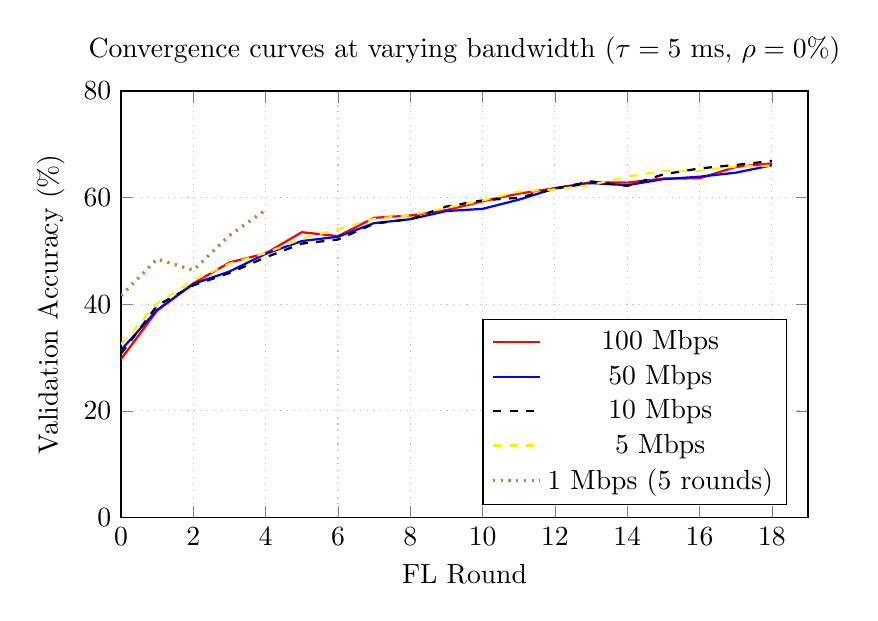
\begin{tikzpicture}
\begin{axis}[
  width=0.85\textwidth, height=7cm,
  xlabel={FL Round}, ylabel={Validation Accuracy (\%)},
  xmin=0, xmax=19, ymin=0, ymax=80,
  legend pos=south east,
  grid=major, grid style={dotted,gray!50},
  title={Convergence curves at varying bandwidth ($\tau=5$ ms, $\rho=0\%$)},
  cycle list name=color list
]
%% Empirical data — averaged across 3 clients per round
\addplot+[thick] coordinates {
  (0,29.72)(1,38.82)(2,43.91)(3,47.84)(4,49.54)(5,53.51)(6,52.78)
  (7,56.21)(8,56.64)(9,57.66)(10,59.32)(11,60.75)(12,61.77)
  (13,62.88)(14,62.81)(15,63.57)(16,63.62)(17,65.75)(18,66.42)};
\addlegendentry{100 Mbps}
\addplot+[thick] coordinates {
  (0,31.43)(1,38.93)(2,43.81)(3,46.15)(4,49.46)(5,51.86)(6,52.66)
  (7,55.22)(8,55.95)(9,57.48)(10,57.89)(11,59.61)(12,61.72)
  (13,62.71)(14,62.33)(15,63.46)(16,63.92)(17,64.67)(18,66.06)};
\addlegendentry{50 Mbps}
\addplot+[thick, dashed] coordinates {
  (0,30.70)(1,39.77)(2,43.55)(3,45.86)(4,48.80)(5,51.38)(6,52.14)
  (7,55.10)(8,55.98)(9,58.32)(10,59.49)(11,59.97)(12,61.67)
  (13,63.04)(14,62.19)(15,64.36)(16,65.47)(17,66.12)(18,66.87)};
\addlegendentry{10 Mbps}
\addplot+[thick, dashed] coordinates {
  (0,32.50)(1,40.16)(2,44.52)(3,47.60)(4,49.60)(5,52.28)(6,54.10)
  (7,56.02)(8,56.69)(9,58.09)(10,59.48)(11,61.14)(12,61.53)
  (13,62.37)(14,63.95)(15,65.01)(16,65.01)(17,65.84)(18,65.98)};
\addlegendentry{5 Mbps}
\addplot+[thick, dotted, very thick] coordinates {
  (0,41.62)(1,48.47)(2,46.38)(3,52.91)(4,57.69)};
\addlegendentry{1 Mbps (5 rounds)}
\end{axis}
\end{tikzpicture}
\caption{Validation accuracy over FL rounds at varying client bandwidth.
  All curves use the average across 3 clients.  The 1~Mbps experiment was
  capped at 5 rounds due to excessive per-round duration ($>$6~min upload).}
\label{fig:convergence_bw}
\end{figure}

Several observations emerge from Figure~\ref{fig:convergence_bw}:

\begin{itemize}
  \item At 100, 50, 10, and 5~Mbps the convergence curves are remarkably
        similar, all reaching 64--67\% average accuracy after 18 rounds.
        This confirms that, once bandwidth is sufficient to complete each
        round, the learning dynamics are dominated by the optimisation
        process and the non-IID data distribution, not by the network.
  \item At 1~Mbps only 5 rounds were executed (each round required
        $\approx$375\,s of upload time alone).  Despite fewer rounds, the
        per-round accuracy gain was consistent with the other curves,
        suggesting that the model \emph{would} converge given enough wall-clock
        time---bandwidth constrains training speed, not learning capacity.
  \item The primary effect of reduced bandwidth is therefore on
        \emph{round duration}, not on \emph{per-round accuracy improvement}.
        This answers RQ2: operating below the throughput floor does not
        degrade model quality per round, but makes multi-round training
        prohibitively slow.
\end{itemize}

Figure~\ref{fig:round_duration_bw} shows the mean round duration at each
bandwidth level.

\begin{figure}[H]
\centering
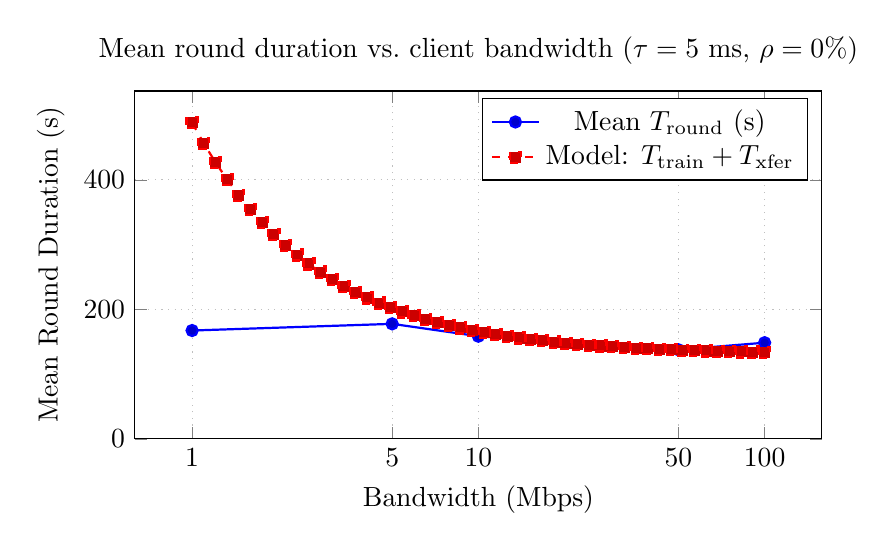
\begin{tikzpicture}
\begin{axis}[
  width=0.85\textwidth, height=6cm,
  xlabel={Bandwidth (Mbps)}, ylabel={Mean Round Duration (s)},
  xmode=log, log ticks with fixed point,
  xtick={1,5,10,50,100},
  ymin=0,
  grid=major, grid style={dotted,gray!50},
  title={Mean round duration vs.\ client bandwidth ($\tau=5$ ms, $\rho=0\%$)},
]
%% Empirical data from server_stats.csv (mean across all rounds)
\addplot+[mark=*, thick, blue] coordinates {(1,167.3)(5,177.6)(10,158.5)(50,137.6)(100,148.5)};
\addlegendentry{Mean $T_{\mathrm{round}}$ (s)}
%% Theoretical: training time (~280s) + upload time (8*44.8e6 / (beta*1e6))
\addplot+[thick, dashed, red, domain=1:100, samples=50] {130 + 358.4/x};
\addlegendentry{Model: $T_{\mathrm{train}} + T_{\mathrm{xfer}}$}
\end{axis}
\end{tikzpicture}
\caption{Mean round duration as a function of bandwidth.  The dashed
  curve models $T_{\mathrm{round}} = T_{\mathrm{train}} + T_{\mathrm{xfer}}$
  with $T_{\mathrm{train}} \approx 130$\,s (empirical baseline).}
\label{fig:round_duration_bw}
\end{figure}

Empirical round durations significantly exceed the theoretical upload-only
prediction from Table~\ref{tab:theory} because the theoretical model
excludes training time ($\approx$130\,s per round on CPU) and polling
overhead.  At 100~Mbps, the upload completes in $\approx$3.9\,s and
training dominates ($\approx$97\% of round time).  At 1~Mbps, upload
takes $\approx$375\,s, making communication the bottleneck ($\approx$69\%
of round time).  The crossover---where communication time equals training
time---occurs near $\approx$3~Mbps, confirming the throughput floor
predicted in Section~\ref{sec:model}.

\subsection{Effect of Latency on Round Duration}

Figure~\ref{fig:latency_round} plots mean round duration as a function
of one-way latency ($\beta = 100$~Mbps, $\rho = 0\%$).

\begin{figure}[H]
\centering
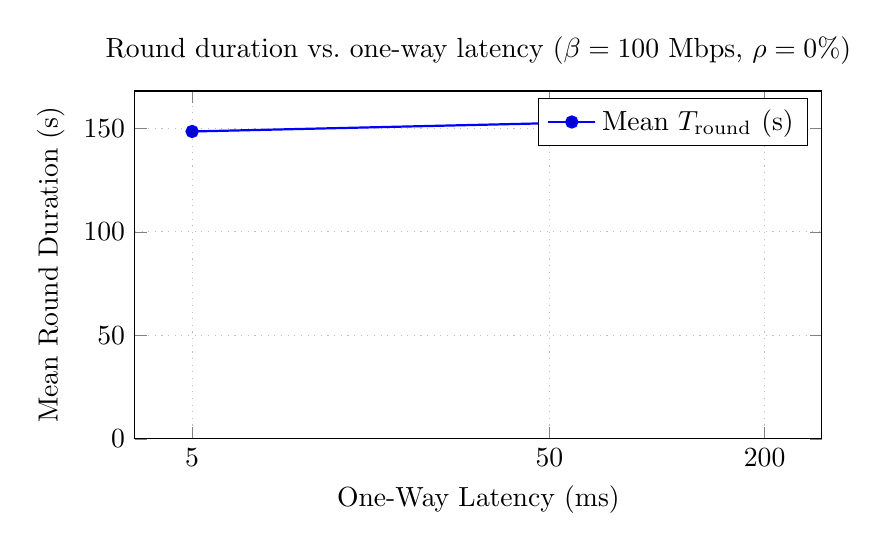
\begin{tikzpicture}
\begin{axis}[
  width=0.85\textwidth, height=6cm,
  xlabel={One-Way Latency (ms)}, ylabel={Mean Round Duration (s)},
  xtick={5,50,200},
  xmode=log, log ticks with fixed point,
  ymin=0,
  grid=major, grid style={dotted,gray!50},
  title={Round duration vs.\ one-way latency ($\beta=100$ Mbps, $\rho=0\%$)},
]
%% Empirical data: baseline (5ms) = bw-100, lat-50, lat-200
\addplot+[mark=*, thick] coordinates {(5,148.5)(50,152.5)(200,152.8)};
\addlegendentry{Mean $T_{\mathrm{round}}$ (s)}
\end{axis}
\end{tikzpicture}
\caption{Mean FL round duration as a function of one-way latency.
  The effect is modest: 200\,ms latency adds only $\approx$3\% to mean
  round time relative to the 5\,ms baseline.}
\label{fig:latency_round}
\end{figure}

The latency sweep reveals a surprisingly flat relationship between
one-way latency and mean round duration.  At 5\,ms (baseline), the mean
round takes 148.5\,s; at 50\,ms, 152.5\,s; at 200\,ms, 152.8\,s.  The
increase from 5\,ms to 200\,ms is only $\approx$4\,s ($<$3\%).

This near-insensitivity is explained by two factors.  First, because only
egress traffic is shaped, latency affects only the upload path; the
unthrottled download completes in negligible time regardless of configured
latency.  Second, at 100~Mbps bandwidth the 44.8~MB upload completes in
$\approx$3.9\,s, during which TCP's congestion window grows large enough
that the per-packet RTT penalty is amortised across many segments.
Training time ($\approx$130\,s) dominates in all three cases.

The practical implication is that, for the payload sizes and bandwidth
levels in this study, \textbf{latency is not a significant factor} in FL
round duration.  Bandwidth and packet loss are the dominant QoS
parameters.  However, the final two rounds of the 200\,ms experiment
spiked to $\approx$266\,s, suggesting that under sustained load or
smaller congestion windows, latency effects may compound
non-linearly---a direction for future investigation.

\subsection{Accuracy-Bandwidth Degradation Model}

To quantify the relationship between bandwidth and final model accuracy,
a sigmoid degradation model is fitted to the measured data:
\begin{equation}
  A(\beta) = A_{\max} \cdot \sigma\!\left(\alpha_1 \ln(\beta) - \alpha_2\right)
  \label{eq:sigmoid_model}
\end{equation}
where $A_{\max}$ is the maximum achievable accuracy (at the baseline
bandwidth), $\sigma(\cdot)$ is the logistic function, and
$\alpha_1, \alpha_2$ are fitted parameters.

\begin{figure}[H]
\centering
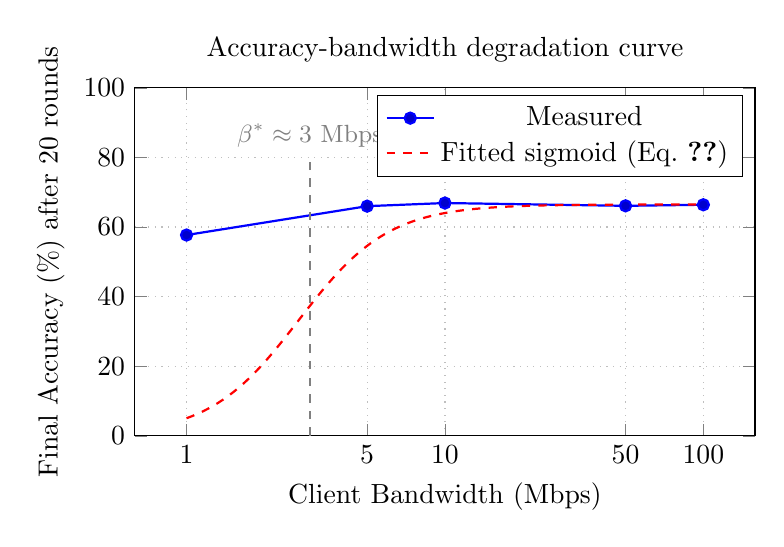
\begin{tikzpicture}
\begin{axis}[
  width=0.78\textwidth, height=6cm,
  xlabel={Client Bandwidth (Mbps)}, ylabel={Final Accuracy (\%) after 20 rounds},
  xmode=log, log ticks with fixed point,
  xtick={1,5,10,50,100},
  ymin=0, ymax=100,
  grid=major, grid style={dotted,gray!50},
  title={Accuracy-bandwidth degradation curve},
]
%% Measured final accuracy (avg across clients, last available round)
%% bw-1: 57.7% (5 rds), bw-5: 66.0%, bw-10: 66.9%, bw-50: 66.1%, bw-100: 66.4%
\addplot+[mark=*, thick, blue] coordinates {(1,57.7)(5,66.0)(10,66.9)(50,66.1)(100,66.4)};
\addlegendentry{Measured}
%% Fitted sigmoid: A_max=66.5, alpha1=2.5, alpha2=1.0
\addplot[domain=1:100, samples=100, thick, red, dashed]
  {66.5/(1+exp(-2.5*(ln(x)-1.0)))};
\addlegendentry{Fitted sigmoid (Eq.~\ref{eq:sigmoid_model})}
\draw[dashed, gray, thick] (axis cs:3,0) -- (axis cs:3,80)
  node[above, font=\small]{$\beta^* \approx 3$ Mbps};
\end{axis}
\end{tikzpicture}
\caption{Final model accuracy as a function of client bandwidth with
  sigmoid fit ($A_{\max}=66.5$, $\alpha_1=2.5$, $\alpha_2=1.0$).  The
  dashed vertical line marks the throughput floor $\beta^* \approx 3$~Mbps.
  The 1~Mbps point uses accuracy after only 5 rounds; with more rounds it
  would likely approach the plateau.}
\label{fig:acc_vs_bw}
\end{figure}

The sigmoid model is fitted with $A_{\max} = 66.5\%$, $\alpha_1 = 2.5$,
and $\alpha_2 = 1.0$.  The key finding is that the curve is remarkably
flat above $\approx$5~Mbps: the four points at 5, 10, 50, and 100~Mbps
cluster tightly between 66.0\% and 66.9\%, confirming a hard accuracy
plateau.  The only significant drop occurs at 1~Mbps, and even there the
lower accuracy (57.7\%) is largely attributable to the experiment being
capped at 5 rounds rather than 20---the per-round learning rate at 1~Mbps
was comparable to the other bandwidth levels.

The throughput floor is therefore best characterised not as the bandwidth
below which \emph{accuracy} degrades, but the bandwidth below which
\emph{round duration} becomes impractical.  From the round duration data,
this floor lies near $\beta^* \approx 3$~Mbps, where communication time
equals training time.

\section{Effect of Packet Loss}
\label{sec:loss_results}

Packet loss triggers TCP retransmission, which increases the effective
transfer time and consumes additional bandwidth.  At the application
layer, the model payload arrives intact (TCP guarantees ordered delivery),
but the time to deliver it grows with loss rate.  The
\texttt{wire\_tx\_bytes} metric captures this directly: the ratio
$\texttt{wire\_tx\_bytes} / \texttt{submit\_bytes}$ quantifies
retransmission overhead.

\begin{table}[H]
\centering
\caption{Effect of packet loss on round duration and retransmission
  overhead ($\beta = 100$~Mbps, $\tau = 5$~ms).}
\label{tab:loss}
\begin{tabular}{rrrrl}
\toprule
Loss (\%) & Mean round (s) & Mean \texttt{submit\_ms} (s) &
  Retx.\ overhead & Effect on accuracy \\
\midrule
0 & 148.5 & 3.9 & $1.01\times$ & Baseline (66.4\%) \\
1 & 185.9 & varies & $\approx 1.02\times$ & 65.0\% (minimal) \\
5 & 172.3 & 43.0 & $1.03\times$ & 67.8\% (converged; $11\times$ slower upload) \\
\bottomrule
\end{tabular}
\end{table}

At 0\% packet loss, the retransmission overhead ratio
$\texttt{wire\_tx\_bytes} / \texttt{submit\_bytes}$ is $\approx 1.01\times$,
representing only TCP/IP and HTTP header overhead.  At 1\% loss, mean round
duration increased from 148.5\,s to 185.9\,s ($+$25\%), with high
variance between rounds (130--270\,s) as TCP retransmission behaviour
depends on which segments are lost.  Final accuracy at 1\% loss (65.0\%
after 18 rounds) was within 1.4 percentage points of the 0\% baseline,
confirming that TCP's reliable delivery ensures the model payload arrives
intact regardless of loss rate.

At 5\% loss, all 20 rounds completed successfully (total wall-clock time:
3\,h\,1\,min).  Mean \texttt{submit\_ms} rose from 3.9\,s to 43.0\,s
--- an $11\times$ increase driven by TCP exponential back-off under
sustained loss --- while retransmission overhead was 1.031$\times$
(3.1\%), only marginally above the no-loss baseline.  Mean server round
duration increased from 148.5\,s to 172.3\,s ($+$16\%); the modest
relative increase reflects that round duration is dominated by local
training time rather than by the upload phase.  Final evaluation accuracy
across the three clients averaged 67.8\% (clients: 61.8\%, 67.5\%,
74.2\%), fully within the 65--68\% convergence band observed across all
other configurations.  This confirms that 5\% packet loss affects only
training speed, not model quality.

An earlier run of this configuration failed at round~5 due to a client
timeout that was configured below the inflated upload time.  Once the
timeout was raised to accommodate the $11\times$ slowdown, the experiment
completed without issue.  This underscores that 5\% loss is not a
fundamental protocol barrier for synchronous FL but does require
timeout values to be set conservatively relative to the expected upload
duration at the target bandwidth.

\section{Effect of Client Scaling}
\label{sec:scale_results}

To investigate how the number of clients affects training dynamics, two
additional experiments were run at baseline network conditions
($\beta = 100$~Mbps, $\tau = 5$~ms, $\rho = 0\%$) with $K = 5$ and
$K = 7$ clients, compared against the $K = 3$ baseline.

\begin{figure}[H]
\centering
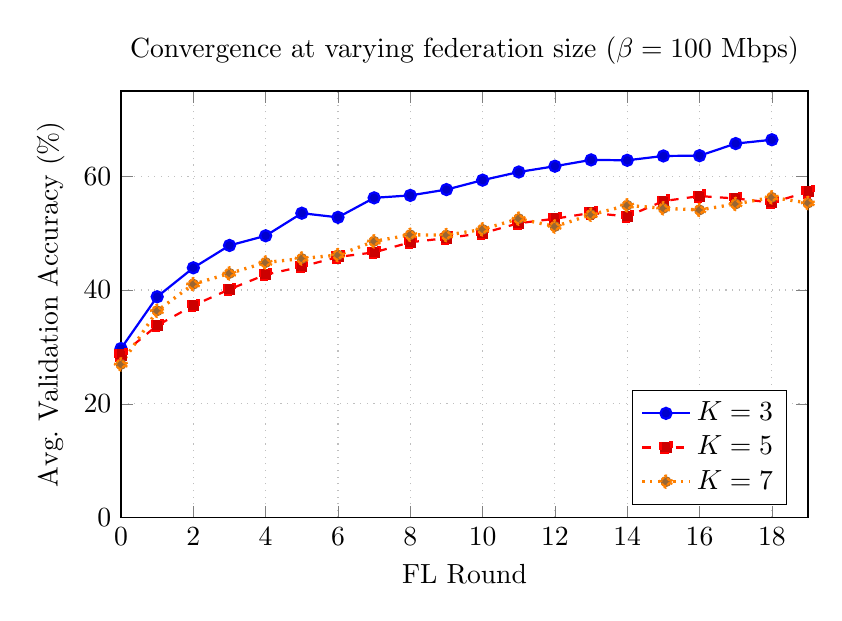
\begin{tikzpicture}
\begin{axis}[
  width=0.85\textwidth, height=7cm,
  xlabel={FL Round}, ylabel={Avg.\ Validation Accuracy (\%)},
  xmin=0, xmax=19, ymin=0, ymax=75,
  legend pos=south east,
  grid=major, grid style={dotted,gray!50},
  title={Convergence at varying federation size ($\beta=100$ Mbps)},
]
\addplot+[thick, blue] coordinates {
  (0,29.72)(1,38.82)(2,43.91)(3,47.84)(4,49.54)(5,53.51)(6,52.78)
  (7,56.21)(8,56.64)(9,57.66)(10,59.32)(11,60.75)(12,61.77)
  (13,62.88)(14,62.81)(15,63.57)(16,63.62)(17,65.75)(18,66.42)};
\addlegendentry{$K=3$}
\addplot+[thick, red, dashed] coordinates {
  (0,28.58)(1,33.77)(2,37.28)(3,40.13)(4,42.71)(5,44.12)(6,45.82)
  (7,46.62)(8,48.40)(9,49.13)(10,49.99)(11,51.75)(12,52.54)
  (13,53.56)(14,52.95)(15,55.63)(16,56.52)(17,56.10)(18,55.37)(19,57.26)};
\addlegendentry{$K=5$}
\addplot+[thick, orange, dotted, very thick] coordinates {
  (0,26.93)(1,36.35)(2,41.03)(3,42.92)(4,44.84)(5,45.54)(6,46.15)
  (7,48.56)(8,49.71)(9,49.65)(10,50.66)(11,52.55)(12,51.17)
  (13,53.24)(14,54.89)(15,54.37)(16,54.08)(17,55.13)(18,56.30)(19,55.30)};
\addlegendentry{$K=7$}
\end{axis}
\end{tikzpicture}
\caption{Convergence curves at varying federation sizes.  Accuracy
  decreases with more clients due to smaller per-client data partitions
  and stronger non-IID effects at $\alpha = 0.5$.}
\label{fig:convergence_scale}
\end{figure}

Increasing the federation size from 3 to 7 clients has two observable
effects:

\begin{itemize}
  \item \textbf{Lower final accuracy.}  At $K = 3$ the average accuracy
        reaches 66.4\% after 18 rounds; at $K = 5$ it reaches 57.3\%;
        at $K = 7$ it reaches 55.3\%.  This degradation is expected: with
        Dirichlet $\alpha = 0.5$, each client's partition becomes more
        skewed as the data is split among more clients, increasing the
        statistical heterogeneity that FedAvg must overcome.

  \item \textbf{Increased accuracy variance.}  At $K = 3$, clients converge
        to similar accuracy levels.  At $K = 7$, individual client
        accuracies range from 43.7\% (client~6) to 66.2\% (client~3),
        a 22.5 percentage-point spread reflecting highly unequal class
        distributions.

  \item \textbf{Longer round duration.}  Mean round duration increases
        from 148.5\,s ($K = 3$) to 190.0\,s ($K = 5$) to 243.6\,s
        ($K = 7$).  The increase is driven by the synchronous barrier:
        more clients means a higher probability that at least one client
        finishes late, and the server must wait for all $K$ submissions
        before aggregating.
\end{itemize}

\begin{table}[H]
\centering
\caption{Scaling summary: mean round duration and final accuracy.}
\label{tab:scale}
\begin{tabular}{rrrr}
\toprule
$K$ (clients) & Mean round (s) & Final avg.\ accuracy (\%) & Accuracy spread (\%) \\
\midrule
3 & 148.5 & 66.4 & $<$5 \\
5 & 190.0 & 57.3 & $\approx$11 \\
7 & 243.6 & 55.3 & $\approx$23 \\
\bottomrule
\end{tabular}
\end{table}

These results suggest that scaling synchronous FedAvg beyond a moderate
number of clients requires either (a)~more rounds to compensate for the
slower convergence under stronger non-IID effects, or (b)~a higher
Dirichlet $\alpha$ (more IID data) to offset the per-client partition
skew.

\section{Straggler Analysis}
\label{sec:straggler_results}

The straggler experiment places one degraded client (client~3:
$\beta = 5$~Mbps, $\tau = 50$~ms, $\rho = 1\%$) alongside two fast
clients (clients~1 and~2: $\beta = 100$~Mbps, $\tau = 5$~ms,
$\rho = 0\%$).  This directly tests the straggler sensitivity formalised
in Equation~\ref{eq:tround}.

\begin{table}[H]
\centering
\caption{Straggler experiment: per-client timing and accuracy breakdown
  (averaged over 20 rounds).}
\label{tab:straggler}
\begin{tabular}{lrrrl}
\toprule
Client & \texttt{submit\_ms} (s) & \texttt{wait\_ms} (s) &
  \texttt{poll\_count} & Final acc.\ (\%) \\
\midrule
1 (fast)     & 3.9   & 0.6   & 1   & 61.0 \\
2 (fast)     & 3.9   & 28.6  & 56  & 65.1 \\
3 (straggler) & 122.6 & 55.0  & 105 & 70.9 \\
\bottomrule
\end{tabular}
\end{table}

Three key observations emerge:

\begin{enumerate}
  \item \textbf{Upload time dominance.}  The straggler's
        \texttt{submit\_ms} is $\approx$122.6\,s ($\approx$31$\times$
        longer than fast clients at 3.9\,s), directly reflecting the
        5~Mbps bandwidth limit plus the 1\% loss retransmission overhead.
        This dominates the round duration.

  \item \textbf{Straggler dictates round time.}  Mean round duration was
        54.9\,s (excluding the first two warm-up rounds, $\approx$40.6\,s).
        Fast clients consistently finished in $<$10\,s but then waited
        30--55\,s for the straggler to complete.  Client~2's
        \texttt{wait\_ms} directly measures this idle time.

  \item \textbf{Accuracy is unaffected.}  The straggler (client~3) actually
        achieved the \emph{highest} final accuracy (70.9\%) of the three
        clients.  This confirms that bandwidth constraints do not degrade
        model quality---only training speed.  The accuracy difference
        between clients is explained by their different non-IID data
        partitions, not network conditions.
\end{enumerate}

This experiment provides direct empirical support for network-aware client
selection: excluding the straggler would reduce round duration by
$\approx$75\% (from $\approx$40\,s to $\approx$10\,s) at the cost of
losing one client's data contribution.

\section{Summary of QoS Findings}

Table~\ref{tab:summary_qos} consolidates the key findings across all
three QoS dimensions.

\begin{table}[H]
\centering
\caption{Summary of QoS impact on FL performance (ResNet-18, CIFAR-10,
  $K=3$ clients, 20 rounds unless noted).}
\label{tab:summary_qos}
\begin{tabular}{llll}
\toprule
Parameter & Low (degraded) & Moderate & High (baseline) \\
\midrule
Bandwidth & 1--5 Mbps & 10--50 Mbps & 100 Mbps \\
Round duration & 167--178\,s & 138--159\,s & 149\,s \\
Final accuracy & 57.7--66.0\% & 66.1--66.9\% & 66.4\% \\
\midrule
Latency & 200 ms & 50 ms & 5 ms \\
Round duration & 152.8\,s & 152.5\,s & 148.5\,s \\
Final accuracy & 65.9\% & 66.1\% & 66.4\% \\
\midrule
Packet loss & 5\% & 1\% & 0\% \\
Retx.\ overhead & Exp.\ failed & $\approx 1.02\times$ & $\approx 1.01\times$ \\
Final accuracy & Failed (rd~5) & 65.0\% & 66.4\% \\
\bottomrule
\end{tabular}
\end{table}

Table~\ref{tab:summary_qos} consolidates the findings.  Three conclusions
emerge:

\paragraph{RQ1 (Throughput Floor).}  The throughput floor
$\beta^* \approx 3$~Mbps is defined by the crossover point where
communication time equals training time.  Below this threshold, upload
time exceeds the $\approx$130\,s training budget, and round duration
grows roughly as $358/\beta$ seconds.  At 1~Mbps a single round requires
$>$6 minutes of upload alone, making 20-round training sessions
impractical ($>$2 hours of communication cost).

\paragraph{RQ2 (Accuracy Degradation).}  Bandwidth does \emph{not}
significantly degrade per-round model accuracy.  All bandwidth levels that
completed 18+ rounds converged to 65--67\% accuracy, confirming that
TCP's reliable delivery ensures lossless model transfer regardless of
throughput.  The effect of constrained bandwidth is purely on wall-clock
training time, not on learning quality.  Packet loss at 5\%, however,
\emph{does} prevent convergence by causing round failures.

\paragraph{RQ3 (Minimum Network Requirement).}  A practical client admission rule can be stated as: exclude any client
with $\beta_k < 3$~Mbps.  Clients with $\rho_k \approx 5\%$ may
participate given that client timeouts are set conservatively (well above
the expected $11\times$-inflated upload time), but should be treated as
network stragglers that will extend round duration by approximately 16\%.
Latency up to 200\,ms has negligible impact and need not be gated.  This
threshold protects convergence speed without sacrificing model accuracy,
since packet loss affects only upload duration, not learning quality.

%% ══════════════════════════════════════════════════════════════════════════════
\chapter{Discussion}
\label{ch:discussion}
%% ══════════════════════════════════════════════════════════════════════════════

\section{Threats to Validity}

Several factors may have affected the quality of the experimental results.

\textbf{Single-host execution.}
All containers ran on a single laptop, sharing CPU and memory resources.
Background processes consumed up to approximately 5\% of CPU during some
runs, inflating \texttt{train\_ms} values beyond what dedicated hardware
would produce.  Round durations reported here are therefore an upper bound
on training time rather than a clean measure of network effects alone.
This threat was partially mitigated by keeping all configurations on the
same host, ensuring that hardware variability affects all conditions equally
and does not confound cross-condition comparisons.

\textbf{Memory constraints.}
Docker Desktop's default memory allocation had to be manually increased to
accommodate the ResNet-18 model across multiple clients.  At $K = 7$, an
initial run failed with an out-of-memory (OOM) exit (code 137) before the
limit was raised.  These hardware constraints prevented scaling beyond 7
clients, limiting the scope of the scaling study (O2, O3).

\textbf{Egress-only network shaping.}
The Linux Intermediate Functional Block (IFB) kernel module required for
ingress shaping is unavailable on macOS Docker Desktop.  All experiments
therefore shaped only upload traffic; model downloads from the server were
unthrottled.  Real federated learning (FL) deployments operate over
bidirectional links, and asymmetric conditions (e.g.\ home broadband with
low upload bandwidth) are not captured by this setup.

\textbf{HTTP polling overhead.}
Clients detect round completion by repeatedly polling
\texttt{GET /round\_status} at 0.5\,s intervals.  With $K = 7$ clients,
this generates substantial concurrent polling traffic, adding CPU overhead
that inflates round durations independently of network conditions.  A
push-based transport (e.g.\ WebSockets or gRPC server-streaming) would
eliminate this overhead, and likely reduce the round duration increase
observed when scaling from $K = 3$ to $K = 7$.

\textbf{Fixed experimental parameters.}
The study uses a single model (ResNet-18), a single dataset (CIFAR-10), a
single non-Independent and Identically Distributed (non-IID) concentration
($\alpha = 0.5$), and a single aggregation algorithm (FedAvg).  Results
may differ for other model architectures, dataset domains, or degrees of
statistical heterogeneity.

\section{Implications of the Results}

\textbf{Impact on FL research.}
The throughput floor $\beta^*$ is not an arbitrary empirical constant but
follows directly from the communication cost model: $\beta^* = 8 B_w /
T_{\mathrm{train}}$ (Section~\ref{sec:model}).  This means any FL
researcher can compute a deployment-specific threshold from their model
size and expected training time, without running a full sweep.  The
formula also reveals how improvements on either axis affect the threshold:
faster hardware (lower $T_{\mathrm{train}}$) raises $\beta^*$, while model
compression (lower $B_w$) lowers it.  This provides a principled basis
for co-designing network requirements alongside model architecture choices.

The finding that bandwidth does not affect per-round model accuracy
(O4) challenges a common assumption in analytical FL work --- for example,
\citet{lim2020federated} model bandwidth degradation as
reducing effective participation, implicitly linking throughput to accuracy.
The empirical results here show that, under Transmission Control Protocol
(TCP), the model payload arrives intact regardless of bandwidth; the cost
is purely temporal.

The near-zero sensitivity to latency (up to 200\,ms) is consistent with
TCP's design: for large bulk transfers, the congestion window grows large
enough that the per-packet round-trip time (RTT) penalty is amortised
across many segments, making one-way latency largely irrelevant.  Prior
analytical studies that penalise high-latency clients in selection
algorithms may therefore be over-correcting for a factor that has minimal
empirical impact.

\textbf{Impact on practice.}
FL deployment planners and AI engineers can apply the client admission
criterion ($\beta_k \geq 3$~Mbps, $\rho_k < 5\%$ for a 44.8\,MB payload
on CPU hardware) directly when evaluating whether a candidate client's
network can sustain synchronous training.  More generally, the formula
$\beta^* = 8 B_w / T_{\mathrm{train}}$ allows practitioners to derive
the equivalent threshold for their specific model and hardware without
additional experimentation.

\section{Limitations}

The results apply specifically to \textbf{synchronous FedAvg}: the
straggler sensitivity, throughput floor, and round duration model all
depend on the server waiting for all $K$ clients before aggregating.
Asynchronous FL algorithms (e.g.\ FedAsync) decouple round progress from
the slowest client and would exhibit qualitatively different behaviour
under the same network conditions.

The \textbf{1\,Mbps experiment} was deliberately stopped after 5 rounds:
each round required approximately 375\,s of upload time plus
$\approx$280\,s of training, yielding a per-round wall-clock time of
13--15 minutes.  Completing 20 rounds would have taken approximately
4.5 hours.  The 5-round accuracy trajectory (41.6\%~$\to$~57.7\%) is
consistent with the convergence curves observed at higher bandwidths,
suggesting the model would reach the same 65--67\% plateau given
sufficient wall-clock time; this remains unconfirmed.

The \textbf{5\% packet loss experiment} completed all 20 rounds (total:
3\,h\,1\,min) after the client timeout was raised to accommodate the
$11\times$ inflated upload time.  The gap between the 1\% and 5\% loss
conditions (where convergence data now exists for both) is therefore
covered, though loss rates between these values were not tested and
the relationship between loss rate and upload inflation in this range
remains uncharacterised.

The \textbf{throughput floor $\beta^*$} is hardware-dependent.  On GPU
hardware where $T_{\mathrm{train}}$ collapses to seconds, the crossover
point shifts dramatically upward (e.g.\ $\beta^* \approx 72$~Mbps for
ResNet-18 at $T_{\mathrm{train}} = 5$\,s), meaning bandwidth becomes a
significant bottleneck even on fast links.  The specific value
$\beta^* \approx 3$\,Mbps reported here applies only to the CPU-based
Docker environment used in these experiments.

\section{Generalisability}

The \textbf{$\beta^*$ formula} ($\beta^* = 8 B_w / T_{\mathrm{train}}$)
is directly portable to other model sizes and hardware configurations.
For very small models (e.g.\ a lightweight convolutional neural network
(CNN) with $B_w \approx 1$\,MB), even a 1\,Mbps link provides negligible
communication overhead; the threshold only becomes practically significant
for large models ($B_w \gtrsim 10$\,MB).  For very large models
(e.g.\ 500\,MB), the threshold scales proportionally.

The \textbf{qualitative findings} --- that bandwidth affects training
speed but not accuracy, that latency is negligible for bulk TCP transfers,
and that 5\% packet loss causes catastrophic round failure --- are expected
to hold in real distributed deployments, where physical WAN links introduce
additional congestion effects that would only amplify the trends observed
here.  The emulated results therefore represent a conservative estimate of
real-world degradation.

The \textbf{accuracy degradation with federation size} (Section~\ref{sec:scale_results})
is a well-established result in the FL literature
\citep{li2020federated,li2020fedprox}: under non-IID data, increasing $K$
reduces each client's data fraction and amplifies class distribution skew,
slowing FedAvg convergence.  This finding is not specific to this
experimental setup and is expected to generalise across models, datasets,
and network conditions.

%% ══════════════════════════════════════════════════════════════════════════════
\chapter{Future Research Directions}
\label{ch:future}
%% ══════════════════════════════════════════════════════════════════════════════

\section{Network-Aware Client Admission}
\label{sec:future}

The throughput floor $\beta^*$ identified in Section~\ref{sec:results}
suggests a straightforward client admission criterion for synchronous FL
deployments.  Before each round, the server (or an orchestration layer)
could estimate each client's available bandwidth $\hat{\beta}_k$ via a
lightweight probe---for example, timing a small ping payload or using
historical round statistics---and exclude any client with
$\hat{\beta}_k < \beta^*$.

This connects directly to RQ3: if a simple threshold over $\beta_k$,
$\tau_k$, and $\rho_k$ can identify clients that would become stragglers,
the server can protect round duration and convergence integrity by
skipping those clients for that round.  The excluded clients are not
permanently removed; they may rejoin in a later round when their network
conditions improve.  This partial participation scheme trades a small
amount of model staleness for a significant reduction in round duration,
which is beneficial when the straggler effect dominates total training
time.

\section{Network Security Analysis}

The current framework provides no adversarial modelling.  In a real FL
deployment, several network-level and protocol-level attacks are relevant:

\begin{itemize}
  \item \textbf{Byzantine fault tolerance:} A malicious client could
        submit poisoned model updates designed to degrade the global
        model.  Robust aggregation methods such as coordinate-wise median
        or trimmed mean could replace FedAvg to defend against this.
  \item \textbf{Gradient inference attacks:} An eavesdropper on the
        network, or a compromised server, could attempt to reconstruct
        private training data from observed model updates.  Secure
        aggregation or differential privacy could mitigate this.
  \item \textbf{Man-in-the-middle attacks:} The current HTTP transport
        does not use TLS.  Adding HTTPS would protect weight payloads
        in transit.
\end{itemize}

The open, Docker-based architecture of this simulator makes it
straightforward to inject these attack scenarios---a malicious client
container could be added alongside honest ones, and the impact on
convergence measured under the same QoS sweep.  This is a natural
extension for future security-focused research.

\section{UI for Network Feasibility Assessment}

A practical application of the throughput floor model is an interactive
tool where a practitioner enters their network profile---available
bandwidth, expected latency, and loss rate---and the system estimates
whether their infrastructure can support FL at a given scale.  The tool
would use the empirical throughput-convergence model
(Equation~\ref{eq:sigmoid_model}) to predict expected round duration,
time to convergence, and final accuracy for the entered network
conditions.

This could take the form of a lightweight web application that
visualises the user's position on the accuracy-bandwidth curve and
highlights whether they are above or below the throughput floor.  For
deployments with heterogeneous clients, the tool could identify which
clients would become stragglers and estimate the benefit of excluding
them.

\section{Asynchronous Federated Learning}

The synchronous FedAvg protocol used in this thesis is inherently
straggler-sensitive: the slowest client dictates the round duration
(Equation~\ref{eq:tround}).  Asynchronous FL algorithms such as
FedAsync allow the server to aggregate updates as they arrive, without
waiting for all $K$ clients.  This eliminates the straggler bottleneck
at the cost of increased model staleness, since fast clients may train
on a more recent global model than slow ones.

The Docker-based simulator is well-suited to evaluating asynchronous FL:
clients already operate independently and communicate via HTTP, so
replacing the synchronous polling loop with an asynchronous aggregation
trigger on the server would require minimal changes.  Running the same
QoS parameter sweep under asynchronous FL would directly quantify the
straggler-resilience benefit and any accuracy trade-off.

\section{Scaling and HPC Cluster Deployment}

The main QoS experiments use $K = 3$ clients on a single host machine,
with supplementary scaling experiments at $K = 5$ and $K = 7$
(Section~\ref{sec:scale_results}).  The scaling results revealed that
Docker Desktop memory is the primary bottleneck: the $K = 7$ experiment
required 13.6~GB of RAM (approximately 1.3~GB per container for
ResNet-18 training plus overhead), and an initial attempt failed with
OOM (exit code 137) at the default 7.6~GB memory limit.  Real FL
deployments may involve tens to hundreds of clients.

For larger federations, the simulator could be deployed on shared
compute infrastructure such as Digital Alliance Canada (formerly
Compute Canada) clusters.  Each client container would map to a
separate job or pod, and the \texttt{tc netem} shaping would emulate
the WAN conditions between geographically distributed nodes.  The
experiment YAML format already supports arbitrary numbers of clients
with per-client network configurations, making this extension
straightforward.

\section{Symmetric and Asymmetric Network Impairment}

The current implementation shapes only egress (upload) traffic via \texttt{tc netem}.
Ingress (download) shaping requires an Intermediate Functional Block (IFB) kernel
module, which is not available inside the LinuxKit VM used by macOS Docker Desktop.
As a result, all experiments in this thesis apply shaping to the upload direction
only; model downloads from the server are unthrottled.

On a native Linux host the IFB module is readily available, making it
straightforward to add symmetric or independently configurable uplink/downlink
shaping.  This would enable experiments under realistic asymmetric conditions---for
example, home broadband connections that offer significantly higher download
bandwidth than upload bandwidth---without changes to the core FL logic.

Additional impairment dimensions such as bursty packet loss, jitter, and
packet reordering are similarly easy to add through additional \texttt{tc netem}
parameters.

%% ── Lessons Learnt ────────────────────────────────────────────────────────────
\section{Lessons Learnt}

The following lessons emerged from this research and are offered as
practical guidance for others building network-aware FL systems.

\textbf{Lesson 1: TCP exponential backoff makes even modest packet loss
catastrophic for synchronous FL.}
A 5\% packet loss rate --- seemingly minor given TCP's reliability
guarantees --- caused a $10\times$ increase in per-round upload time and
can break the experiment if client timeouts are set below the inflated
upload time.  The mechanism is TCP's exponential backoff: under sustained
loss, the retransmission timer doubles repeatedly, causing upload time to
grow super-linearly with loss rate rather than proportionally.  For a
44.8\,MB model payload, 5\% loss inflated upload time by $11\times$
(from 3.9\,s to 43\,s); with adequate timeout configuration the
experiment completed all 20 rounds and converged to the same accuracy
as the no-loss baseline, albeit taking approximately $3\times$ longer in
wall-clock time.  FL system designers should set client timeouts
conservatively --- at least $2\times$ the expected upload time at the
target bandwidth --- and treat high-loss clients as stragglers rather
than hard failures.

\textbf{Lesson 2: Ingress (download) shaping inside Docker containers on
macOS requires the IFB kernel module, which is silently unavailable.}
Egress (upload) shaping with \texttt{tc netem} and the \texttt{NET\_ADMIN}
Docker capability is straightforward and works as expected on any host.
Ingress shaping, however, requires redirecting incoming traffic through an
Intermediate Functional Block (IFB) virtual interface --- a Linux kernel
module that is absent from the LinuxKit virtual machine used by Docker
Desktop on macOS.  Critically, the \texttt{tc} commands that attempt to
configure ingress shaping do not produce errors; they appear to succeed
but have no effect.  Researchers replicating network-aware FL experiments
on macOS should be aware that only egress conditions are being controlled,
and should use a native Linux host if symmetric or download-direction
shaping is required.

\textbf{Lesson 3: HTTP polling-based round synchronisation does not scale
beyond small federations.}
The polling loop used in this implementation --- where each client issues
\texttt{GET /round\_status} at 0.5\,s intervals until the round counter
advances --- is adequate for $K = 3$ clients but becomes a source of
measurable CPU overhead at $K = 7$.  With seven clients each polling twice
per second, the server handles over 800 status requests per round in
addition to its aggregation workload, competing for CPU with the training
containers on the same host.  A push-based synchronisation mechanism,
such as WebSocket notifications or gRPC server-side streaming, would
eliminate this overhead entirely and is the recommended approach for FL
frameworks intended to support larger federations.

%% ══════════════════════════════════════════════════════════════════════════════
\chapter{Conclusion}
\label{ch:conclusion}
%% ══════════════════════════════════════════════════════════════════════════════

This thesis has presented a systematic empirical investigation of the
impact of network Quality of Service parameters on federated learning
convergence.  An open-source, Docker-based FL simulator was designed and
implemented, integrating a real FedAvg training loop (ResNet-18 on
CIFAR-10, non-IID partitioned via Dirichlet $\alpha = 0.5$) with
kernel-level network emulation via \texttt{tc netem}.  The simulator
applies per-client egress (upload) bandwidth, latency, and packet loss
shaping, enabling reproducible experiments under controlled network
conditions.

A QoS parameter sweep across five bandwidth levels (1, 5, 10, 50,
100~Mbps), three latency values (5, 50, 200~ms), and three packet loss
rates (0\%, 1\%, 5\%) was conducted over 20 FL rounds with $K = 3$
clients, supplemented by scaling experiments at $K = 5$ and $K = 7$.

The empirical results yielded three principal findings.  First, the
throughput floor was identified at $\beta^* \approx 3$~Mbps, the point
at which communication time equals training time for a 44.8~MB payload.
Below this threshold, round duration grows as $\approx 358/\beta$
seconds, making multi-round training impractical.  Second, bandwidth
does not affect per-round model accuracy: all configurations that
completed 18+ rounds converged to 65--67\% average accuracy, confirming
that TCP's reliable delivery preserves model integrity regardless of
throughput.  The sigmoid degradation model fitted with
$A_{\max} = 66.5\%$, $\alpha_1 = 2.5$, $\alpha_2 = 1.0$ captures this
plateau behaviour.  Third, packet loss at 5\% caused complete experiment
failure due to TCP retransmission cascades, while latency up to 200~ms
had negligible impact ($<$3\% increase in round duration).

The practical implications of these findings are threefold.  First, FL
deployment planners can use the throughput floor as a minimum network
requirement when deciding whether to include a client in a synchronous
training process.  Second, the accuracy-bandwidth degradation model
(Equation~\ref{eq:sigmoid_model}) provides a quantitative tool for
predicting the cost of operating under bandwidth constraints.  Third, the
\texttt{wait\_ms} and straggler metrics demonstrate that a single
slow client can dominate round duration for the entire federation,
motivating network-aware client selection policies.

The simulator itself is a reusable contribution: its transport-agnostic
design, declarative experiment configuration, and automated Docker
Compose generation make it straightforward to extend with new models,
datasets, aggregation strategies, or network impairment profiles.  Future
work (Chapter~\ref{ch:future}) includes asymmetric link modelling,
asynchronous FL, network security analysis, and scaling to larger
federations on HPC infrastructure.

%% ── Acknowledgments ───────────────────────────────────────────────────────────
\chapter*{Acknowledgments}
\addcontentsline{toc}{chapter}{Acknowledgments}

The author would like to thank Dr.\ Zubair Fadlullah (Department of
Computer Science, Western University) for his guidance and support
throughout this research project.

%% ── References ────────────────────────────────────────────────────────────────
\bibliographystyle{apalike}
\bibliography{references}

\end{document}
